% This document provides the style to be used for a MSc Thesis at the
% Parallel and Distributed Systems group
\documentclass[11pt,twoside,a4paper,openright]{report}

% use babel for proper hyphenation
\usepackage[british]{babel}
% Graphics: like the DUT logo on the front cover
\usepackage[dvips]{graphicx}
%Enables [H] for figures.
\usepackage{float}
% FONT: times
\usepackage{times}
% for url's use "\url{http://www.google.com/}"
\usepackage{url}
% To allow margin adjustments
\usepackage{changepage}
% To allow listings.
\usepackage{listings}
% To inserts to do's
\usepackage{todonotes}

\begin{document}

%%%%%%%%%%%%%%%%%%%%%%%%%%%%%%%%%%%%%%%%%%%%%%%%%%%%%%%%%%%%%%%%%%%%%%%%%%%%%%%
\hoffset=1.63cm
\oddsidemargin=0in
\evensidemargin=0in
\textwidth=5in

%%%%%%%%%%%%%%%%%%%%%%%%%%%%%%%%%%%%%%%%%%%%%%%%%%%%%%%%%%%%%%%%%%%%%%%%%%%%%%%
\parindent=1em

\pagestyle{empty}

% FRONTCOVER
\begin{titlepage}

\null\vfill

\begin{center}
\LARGE{MultiChain:\\
       		An incremental step in a new distributed data structure}
\end{center}

\vspace{1.5cm}

\begin{center}
Steffan D. Norberhuis\\
steffan@norberhuis.nl
\end{center}

\vfill

\begin{figure}[!b]
\centering
\includegraphics[width={0.5\textwidth}]{pics/TUD_logo_color.eps}
\end{figure}

\vspace{2.0cm}

\end{titlepage}


% EMPTY PAGE
\cleardoublepage

\pagestyle{plain}

% TITLE PAGE: page i (hidden)
\include{titlepage}

% GRADUATION DATA AND ABSTRACT: pages ii and iii (hidden)
%De aankondiging bevat de spreker, titel, plaats, datum en tijd, samenstelling van de afstudeercommissie en een korte samenvatting (maximaal 25 regels).
\thispagestyle{empty}

\noindent \textbf{Author}\\
\begin{tabular}{l}
Steffan D. Norberhuis\\
\\
\end{tabular}\\
\noindent \textbf{Title}\\
\begin{tabular}{l}
MultiChain: an incremental step in a new distributed data structure\\
\\
\end{tabular}\\
\noindent \textbf{MSc presentation}\\
\begin{tabular}{l}
% <MM> DD, YYYY (like \today)
%TODO: #36 GRADUATION DATE\\
\\
\end{tabular}

\vspace{1.1cm}

\noindent \textbf{Graduation Committee}\\
\begin{tabular}{ll}
%TODO: #37 GRADUATION COMMITTEE & Delft University of Technology \\
% The order of listing the names: Graduation prof, supervisor(s), others ordered by title + alphabetical
%examples:
%prof. dr. ir. H. J. Sips (chair) & Delft University of Technology \\
%ir. dr. D. H. J. Epema           & Delft University of Technology \\
Prof. dr. ir. H. J. Sips            & Delft University Of Technology \\
dr. ir. J. A. Pouwelse        & Delft University of Technology \\
dr. ir. Z. Erkin              & Delft University of Technology \\
\end{tabular}

\begin{abstract} %de abstract bevat alleen een korte samenvatting van de inhoud van het onderzoek
Peer-to-peer networks are often large, collaborative networks where peers can join openly.
In these networks peers help other peers often in singular interactions and without direct reciprocity.
Peers can abuse and freeride.
The network without measures can fall into a tragedy of the commons
where no one helps another and only takes advantage of the generousity of peers.
Only if the reputation of a peer is publicly available at scale and tamper proof can a peer-to-peer network
escape the problems of freeriding and attain high utility for all participants.

This thesis focuses on creating the first step for a tamper proof reputation system within Tribler.
Tribler is a peer-to-peer BitTorrent system developed at the Delft University of Technology.
This first step, made by this thesis, is to design and implement a proof-of-concept bookkeeping system MultiChain.
MultiChain tracks the upload and download amounts of peers to eliminate free riding.
This bookkeeping system has to be scalable to be able to process enough transactions.

A new design of a distributed data structure that can be used as a ledger is introduced by this thesis.
This first step with MultiChain is already more resiliant to tampering than previous work.
The design of MultiChain is to have a chain of blocks for every peer.
A block contains a transaction shared between a peer.
This makes both chains of the peers intertwined and entangled between peers.
Abandoning a global ledger leads to a scalable data structure.
The implementation of the design is tested and experimented with within this thesis to validate it to correctly work.
Furthermore, a number of weak points are discussed that are future steps in creating a tamper proof reputation system.

\end{abstract}

\clearpage



\pagenumbering{roman}
\setcounter{page}{4}

% EMPTY PAGE: page iv
\cleardoublepage

% OPTIONAL QUOTATION: page v
%\include{quotation}
% EMPTY PAGE: page vi
%\cleardoublepage

% PREFACE: page v
\chapter*{Preface}
\addcontentsline{toc}{chapter}{Preface}
The huge increase in Bitcoin adoption, 
due to the increase in uncertainty in the security of traditional currency 
after the financial crisis in 2008, 
is only rivaled by the speculation of the enormous possibilities 
of the underlying technology of the blockchain.
The blockchain is the first technology, seen with real world adoption,
that allows to register transactions without a trusted third party.
But the blockchain has several limitations in scalabillity 
that will limit Bitcoins in fully replacing traditional currencies with a digital currency.
It also limits blockchain as a scalable basis for a large scale reputation system, 
similair to a digital currency, with vast amounts of transactions.
This motivated to research the properties and possibilities of a variant of the blockchain:
multichain.

\vspace{1\baselineskip}

\noindent
I would like to acknowledge several people that helped me during my master thesis.
First I would to heartly thank dr.ir. Johan Pouwelse for his mentoring and helping me in setting goals and achieving these goals in a timely manner.
Furthermore I would like to thank dr.ir. Cor-Paul Bezemer for his guidance and help with implementing within Tribler. 
I also would like to thank Elric Milon and Lipu Fei for answering countless questions and problems I encountered durng the programming phase of my thesis.
For the excellent feedback and help to improve my code I would like to thank dr.ir. Niels Zeilemaker.
I am also very thankful for the companionship I felt within my work room 
and I would like to thank especially Hans Bogerts BSc, Niels Doekeijmeier BSc and Ernst van der Hoeven BSc.
You certainly made my work more enjoyable.
Lastly I want to thank the trainers at the Sports and Culture Centre of the Delft University of Technology for giving an challenging outlet outside of my master thesis.

\vspace{1\baselineskip}

\noindent
Steffan Derk Norberhuis

\vspace{1\baselineskip}

\noindent
Delft, The Netherlands

\noindent
\today

% EMPTY PAGE: page vi
\cleardoublepage

% TABLE OF CONTENTS: starting at page vii
\setcounter{tocdepth}{1}
\tableofcontents

\cleardoublepage

\pagenumbering{arabic}
\setcounter{page}{1}




% CHAPTERS ... For instance: History/Prior Work, Design/Implementation, Experiments
% INTRODUCTION
\chapter{Introduction}
\label{chp:introduction}
Tribler is a peer-to-peer file sharing program developed by the Delft University of Technology for research purposes.
Tribler expands the BitTorrent protocol and has added multiple improvements on this protocol.
The main focus of Tribler is to make security and privacy the default for Internet users and impossible to shutdown.
A fully distributed program, not relying on any central component, is needed to achieve this.
Tribler has been designed and build using this methodology\cite{Pouwelse-tribler}\cite{Bakker-tribler}.
This master thesis was conducted as part of the research mission to improve Tribler.

\vspace{1\baselineskip}

\noindent
TODO ORGANISATIONAL DESCRIPTION OF THESIS


%Problem description
\chapter{Problem Description}

The current Bitcoin protocol is depended on the block chain. 
Using a block chain limits Bitcoin in several ways.
These limitations on Bitcoin can be seen as the initial motivation 
for our work to improve the block chain.
But block chain and our improvement can be used in several other fields as well.

Bitcoin and how it uses the block chain technology will be introduced first.
After that the limitations imposed by the block chain will be explained.
Finally an overview will be given of how block chains and our improvements can be used in other fields.

\section{Bitcoin}
The core of the Bitcoin protocol is the block chain.
The block chain contains every transaction of bitcoins.

A transaction consists of three parts.
The public key of the new owner of the bitcoin,
the hash of combination of the previous transaction together with the public key of the new owner,
and the signature of the hash of the current owner.
The previous transaction is a transaction of the same bitcoin.
The ownership of the bitcoin by the current owner can be verified
by verifying the whole history of the bitcoin.
A transaction is usually shortend to Tx in Bitcoin related work and is used in images in this report.

\begin{figure}[H]
	\centerline{\includegraphics[scale=0.3]{problemDescription/figs/transactions.eps}}
	\caption{Transaction chain}
\end{figure}

Multiple transactions are aggregrated into a single block.
The next block is chained to the previous block by adding the hash of the previous block.
These blocks are created by nodes in the network, so called miners.
A miner receives transactions from other nodes in the Bitcoin network.
But the transactions are received in a non deterministic way induced by network characteristics.
The non deterministic nature causes blocks to differ from miner to miner.
The order of transactions has to be agreed upon by the network to eliminate this inconsistentcy.

Bitcoin uses election based upon Proof-Of-Work system.
To every block a nonce is added. 
This nonce is just a number that can be varied,
but is only sound if the result of the hash of the whole block starts with a certain number of zeros.
The amount of zeros required will be discussed later.

%Related work
\chapter{Related Work}
In this chapter we will discuss related work on tamper-proof interaction histories.

\section{Block chain}
\label{sect:bitcoin}
Bitcoin is a digital currency that uses a global, full transaction history
to keep track of transactions made between nodes.
It is called a global, full transaction history,
because the transaction history is shared between every peer and contains every transaction.
The transaction history is a datastructure called the block chain.

The block chain imposes limits on Bitcoin in several ways.
These limitations on Bitcoin can be seen as the initial motivation for our work.
How Bitcoin uses the block chain technology will be introduced first.
In the following sections the limitations imposed by the block chain will be explained.

We will only introduce how Bitcoins uses the block chain and why it does so.
The best starting point for a full explanation of Bitcoins
is the original paper by Nakamoto~\cite{Nakamoto-bitcoin}.

\subsection{Transfer of ownership of a bitcoin}
The core of the Bitcoin protocol is the block chain.
The block chain contains transactions of bitcoins.
We will first describe how the transactions are build up
and later how they are part of the block chain.

A transaction consists of three parts.
The first part is the public key of the new owner of the bitcoin.
The hash of the whole, previous transaction and the public key of the new owner is concatenated.
This concatenation is hashed and this hash is the second part of the transaction.
The final part is the signature by the current owner of this new hash.
Inclusion of the hash of the previous transaction chains a transaction to the previous transaction.

The previous transaction is a transaction of the same bitcoin.
The ownership of the bitcoin by the current owner can be verified
by verifying the whole chain of ownership of the bitcoin.
A transaction is usually shortend to Tx in Bitcoin related work and is used in images in this report.
In Figure \ref{fig:bt-transaction-chain} a diagram can be seen of how transactions are chained.

\begin{figure}
	\centerline{\includegraphics[scale=0.3]{relatedWork/figs/transactions.eps}}
	\caption{Transfer of ownership of bitcoin in a transaction chain.}
	\label{fig:bt-transaction-chain}
\end{figure}

\subsection{Block chain}
Multiple transactions are aggregrated into a single block.
Every block contains the hash of the previous block.
This creates the block chain.
Transaction chains span across several blocks inside the block chain.
A diagram can be seen in Figure \ref{fig:bt-block-chain} of the block chain.

\begin{figure}
        \centerline{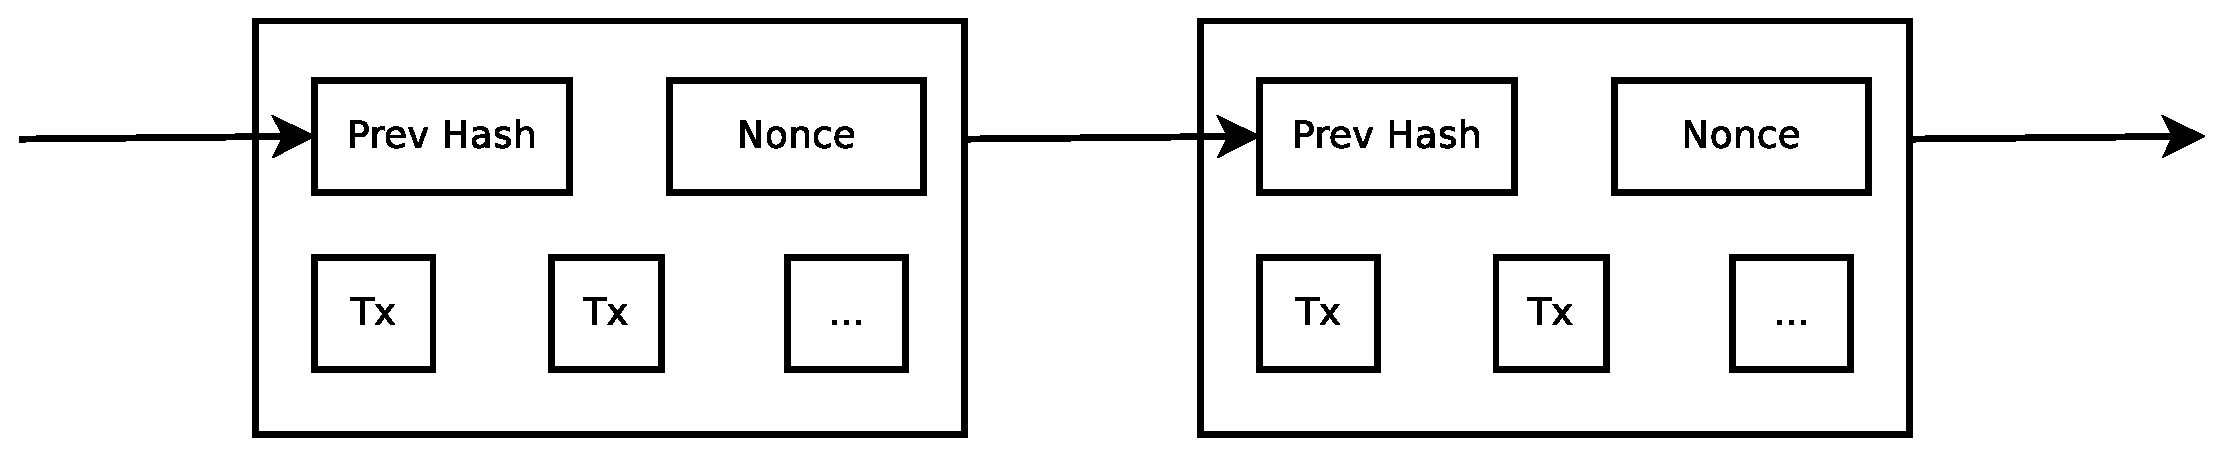
\includegraphics[scale=0.3]{relatedWork/figs/blocks.eps}}
        \caption{Block chain}
        \label{fig:bt-block-chain}
\end{figure}

These blocks in the block chain are created by nodes in the network, so called miners.
A miner receives transactions from other nodes in the Bitcoin network.
An attacker could malicously transmit transactions to double spend a bitcoin he owns or does not have.
So every transaction is verified on arrival at a node.
Any transaction that double spends a bitcoin is simply dropped by the node.
No penalty is awarded to the malicous attacker.

The transactions are received in a non deterministic way induced by network characteristics.
The non deterministic nature causes blocks to differ from miner to miner.
The order of transactions has to be agreed upon by the network to eliminate this inconsistency.

Bitcoin uses election to pick the next block based upon a Proof-Of-Work system.
A nonce is added to every block.
This nonce is just a number that can be varied,
but is only sound if the hash of the whole block starts with a certain number of zeros.
Miners have to find the correct nonce for their block and this is a proof of work.

However, miners can still find a valid nonce at approximately the same time
and notify parts of the network of their newly found block.
This also leaves the network in an inconsisted state.
Multiple versions of the next block attached to the previous block can be seen as branches.

To solve this inconsistency, Bitcoin nodes save both branches and continue using the longest branch.
At some point one branch will become predominant in the network.
More nodes will dedicate compute power to extend this branch and the growth rate will increase for this branch.
The faster growth rate will ensure that the branch will be adopted by the network as a whole.
The smaller branch is abandoned and the blocks are orphaned.

The amount of zeros, needed in the hash of the transaction,
is adjusted to compensate for the fluctuating speed of the network to be able to find nonces.
The speed of the network is called the hash rate and is the amount of hashes calculated per second.
The amount of zeros balances the probability of branches occuring
and the time before a new block is found,
which in turn is how fast transactions are processed.
The amount of zeros can be seen as the difficulty~\cite{bitcoin-difficulty} of finding the a block.
More zeros decreases the likelyhood a nonce will be valid.
The estimated hash rate over time can be seen in Figure \ref{fig:hash-speed}~\cite{Blockchain.info-hashspeed},
and the difficulty in Figure \ref{fig:hash-difficulty}~\cite{Blockchain.info-difficulty}.

\begin{figure}[h]
        \centerline{\includegraphics[scale=0.5]{relatedWork/figs/hashspeed/hashspeed.eps}}
        \caption{Estimated amount of hashes per second.}
	\label{fig:hash-speed}
\end{figure}

\begin{figure}
        \centerline{\includegraphics[scale=0.5]{relatedWork/figs/difficulty/difficulty.eps}}
	\caption{The difficulty of finding blocks.}
	\label{fig:hash-difficulty}
\end{figure}

Another possible attack to double spend a bitcoin is by sending a transaction to one part of the network,
but to the other part of the network a transaction with a different receipient.
It is possible that both transactions will be introduced into the block chain, but in different branches by two independend miners.
Eventually one branch will win and the attack is averted.

The behaviour just described causes that a transaction can never be confirmed with full certainty.
The possibility always exists that another branch over takes the current longest branch.
This makes the network vulnerable if the total compute power is owned by a malicous attacker is more than the total compute power of the honest nodes,
even if the attacker only has control of 51\% of the compute power.
In the end the current branch can be overtaken by a new branch started by the attacker.
This new branch allows the whole transaction history to be rewritten by the attacker.

\subsection{Limitations}
In this section we will discuss the several limitations of Bitcoins
that originate from the use of the block chain.

\subsubsection{Size}
\label{bitcoin-limit-size}
To be able to prevent double spending and enable rightful spending by the owner,
the node verifying a transaction needs to be aware of the full history of a bitcoin.
This results in that a node needs the entire block chain.

The block chain is a data structure ever increasing in size.
No block or data contained in that block is removed.
The block chain has been growing since its inception in 2009.
The size and growth can be seen in Figure \ref{fig:bc-size}.

\begin{figure}
        \centerline{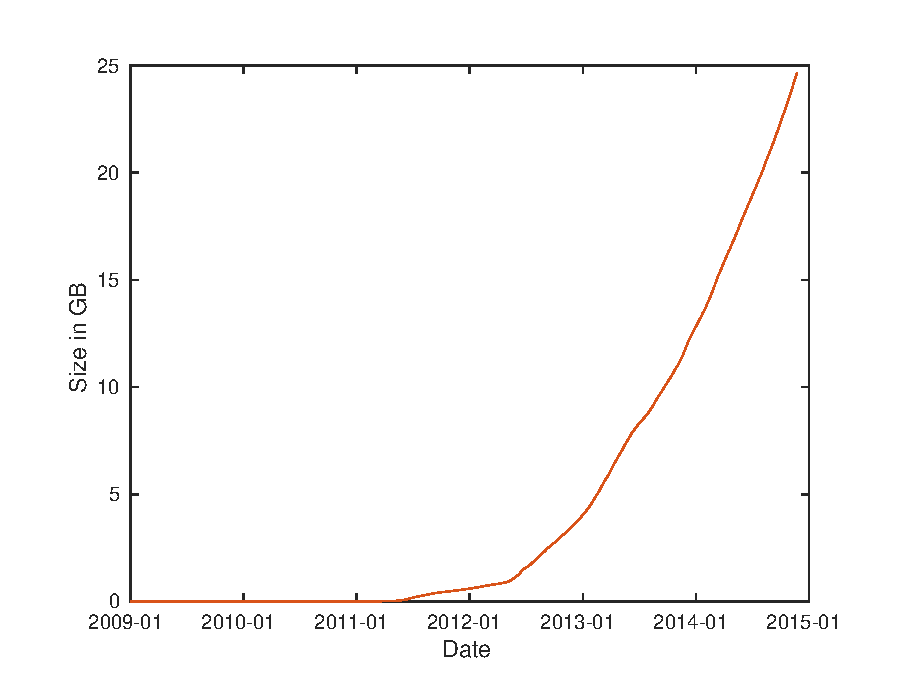
\includegraphics[scale=0.6]{relatedWork/figs/blockchainsize/blockchainsize.eps}}
        \caption{The size of the block chain~\cite{Blockchain.info-bcs}.}
	\label{fig:bc-size}
\end{figure}

The size of the block chain at time of writing already prevents less powerful devices, like smartphones,
to operate on the block chain.
This problem is only going to become bigger with the continued creation of transactions
and at a faster pace due to increased adoption of Bitcoin.
The growth of the size of the block chain has already outpaced the growth of the power of a smartphone
and will also be relatively larger compared to other types of hardware.

This problem was already identified by Nakamoto in his original paper on Bitcoin.
The paper proposes Simplified Payment Verification (SPV).
In SPV mode a node only downloads the block headers of the longest chain.
If a transaction is to be verified, it requests from the network the specific transaction
along with a Merkle tree linking it to a block in the chain.
The Merkle tree can be used to verify that the transaction was included into the block chain.
This allows to calculate with some confidence that the transaction was accepted.

SVP only gives reasonable confidence and is not as secure as running a full node.
Trust has to be placed in the nodes that send the block headers and Merkle Trees.
Secondly, a transaction that is recorded in a more recent block is less difficult to tamper with
than a transaction deep down in the block chain.
This is only an acceptable solution for clients willing to accept more risk due to having a less secure system.
Therefor it is not a solution for the problem for every one.

\subsubsection{Amount of transactions}
The usability of a digital currency is in part determined by the time it takes to process a transaction
and how many transactions can be processed in a certain time scale.
The amount of transactions that can be handled by Bitcoins are determined by two factors:
\begin{itemize}
\item Block size
\item Block creation time
\end{itemize}

The block size is currently capped at a fixed maximum size.
A block can be smaller, but cannot exceed the maximum size.
The current blocksize limit is 1MB.
A block has a fixed part and the rest is filled up by transactions picked by the miner.
A transaction can vary in length.
The number of transactions that can be fitted inside a block is limited by the maximum size.

This maximum size has no clear documentation of why it was picked as such.
There are several implications of raising the size, aswell as lowering.
Increasing the block size will increase the number of transactions that can be processed.
But the increased block size will increase propogation time of the block in the network.
A longer propogation time will in turn result in a higher orphane rate of the miner.

Large clusters of hash power owned by a single miner or mine cluster can be placed closer together
reducing propogation time for this miner.
This will benefit this single miner in reducing his orphaned rate
and will increase the chance of his block being adopted.
This will make the network as a whole more susptible to attack by a single powerful miner
and will reduce the power of other miners.

The difficulty of finding a new block roughly regulates how fast new blocks are created.
The difficulty is set according to the hash rate of the whole network to equal roughly a new block every 10 minutes.
If the time of finding a new block is decreased,
then more blocks are generated and obviously more transactions can be fitted inside these blocks.
The reverse is true if the time is increased.
But the time between blocks is a balance between the orphan rate of blocks
and how fast transactions are committed to the block chain.

These two factors currently result in a theoretical limit of 7 transactions per second~\cite{bitcoin-transactions}.
This can be calculated by dividing the maximum blocksize with the minimal size of a transaction.
The performance of Bitcoin can be changed by changing the settings of these two factors.
This limits the global usage of Bitcoins.
In comparison, Visanet, that handles transactions under Visa,
is able to process 54.000 transactions per second~\cite{visa-transactions}.
To be a real replacement of the current traditional currencies
a higher number of transactions per second have to be achieved by a digital currency.
There are at time of writing several competing proposals to increase the block size~\cite{garzik-blocksize,andresen-blocksize}.



\input{relatedWork/bartercast.tex}

\subsection{Other related work}
The topic of reputation system is currently a subject of research for other projects as well.
There are two more projects worth to briefly mention because of similairity to the Tribler project
and the struggle to build a reputation system.
These projects are not so thoroughly explained as the blockchain
as they were not used as a starting point in designing MultiChain.
The Tor project is working on a implementation of a reputation system
in an effort to incentivize collaboration\cite{androulaki-torincentive}\cite{chen-torincentive}\cite{dingledine-torincentive}\cite{ghosh-torincentive}\cite{jansen-torincentive}.
The InterPlanetary File System \(IPFS\) is a peer-to-peer distributed file system with similairities to the Tribler project.
IPFS uses an incentivized block exchange to improve collaboration\cite{benet-ipfs}.
%Design
\chapter{Design and implementation}
This chapter contains the design of MultiChain and how it was implemented.
We will describe how MultiChain is part of Tribler and its main pillar of design.
The contents of blocks are presented and how they form chains in MultiChain.
We will cover the creation of blocks and the multiple implications of the chosen design.
Additional pheripheral systems that work with MultiChain are also explained.

\section{MultiChain Community}
Tribler uses communities to add functionalities to peers.
A peer loads in a community and this community provides a set of messages and endpoints for other peers.
The community can communicate with the endpoints of other peers as well and send a message to these endpoint.
Other peers are automatically discovered using Dispersy.
Examples of a community are the TunnelCommunity that adds functionality to download anonymously\cite{Plak-anonymous}
or the AllChannelCommunity to distribute torrent files.
The designed system will be implemented by adding a new community to Tribler.

The MultiChain community can be run standalone,
but its main use is to integrate with Tribler and track up and download for torrents.
It will replace the current reputation system Bartercast in the future.
\section{Abandoning full transaction history distribution}
One of the main pillars of the design is to have a transaction history for every peer.
This is in contrast to not distribute a common, full transaction history containing the transactions of every peer.
For example used in the design of the blockchain of Bitcoins, discussed in section \ref{sect:bitcoin}.
The reasoning behind the idea to abandon is that a common, full truth
will become the bottleneck in the system.
This will limit the amount of interactions that can be processed
or will limit the participiation of less powerfull machines.

The reason for the limitation is that every interactions will have to be distributed to every peer in the network.
Every transaction has to be processed by every node at the cost of bandwidth, compute power and storage.
The cost might be very limited for a single transaction,
but with greater scale these cost will add up.
The amount of these three resources is limited and will limit the amount of transactions that can be processed.
This problem can be seen to affect Bitcoins and has been demonstrated in section \ref{bitcoin-limit-size}.

Every node has its own transaction history and only needs the transaction history of its peers it interacts with.
The amount of bandwidth, compute power and storage is limited to the minimal needed amount
that is needed to process only the relevant transactions.
This should allow low-powered devices to keep participating when they only have a low volume of transactions.
It also allows higher volumes of transactions in the system as a whole.
\section{Transactions}
A peer will have transactions with other peers in the network.
The peer will want to have an increase in his reputation and have a transaction be created.
The transaction contains the information about how much data was uploaded and downloaded between the peers
and their total upload and download amounts.

The transaction will be encapsulated inside a single block.
A block contains both public keys of the peers,
so it is possible to see between which peers the transaction is.
Both peers sign the block to acknowledge that the transaction has happened.
Every block only contains one transaction.

The blocks are linked to previous blocks by adding the hashes of the previous blocks of both peers.
This creates a directed acyclic graph of blocks.
A chain can be identified within this graph for every peer.
This chain contains every transaction of a peer.

An example of three blocks can be seen in Figure \ref{fig:chain-example}.
The arrows denote the corresponding hash or signature.
In this example the first block is between peer B and C.
The block contains hashes to the previous blocks of both B and C
and can be seen by the outward arrows.
Inside the block it can be seen what part peer B and C signs by the boxes.
The whole block is not signed by both parties.
The reason for this is explained in section \ref{design:block_creation}.

In the example both peer B and C also conduct a transaction with another peer, A and D respectively.
This creates two new blocks and are chained to the block between B and C by adding the previous hash to the new blocks.
The new blocks also contains the previous hashes of A and D
and chain the new block to previous blocks of A and D.

\begin{figure}
	\centerline{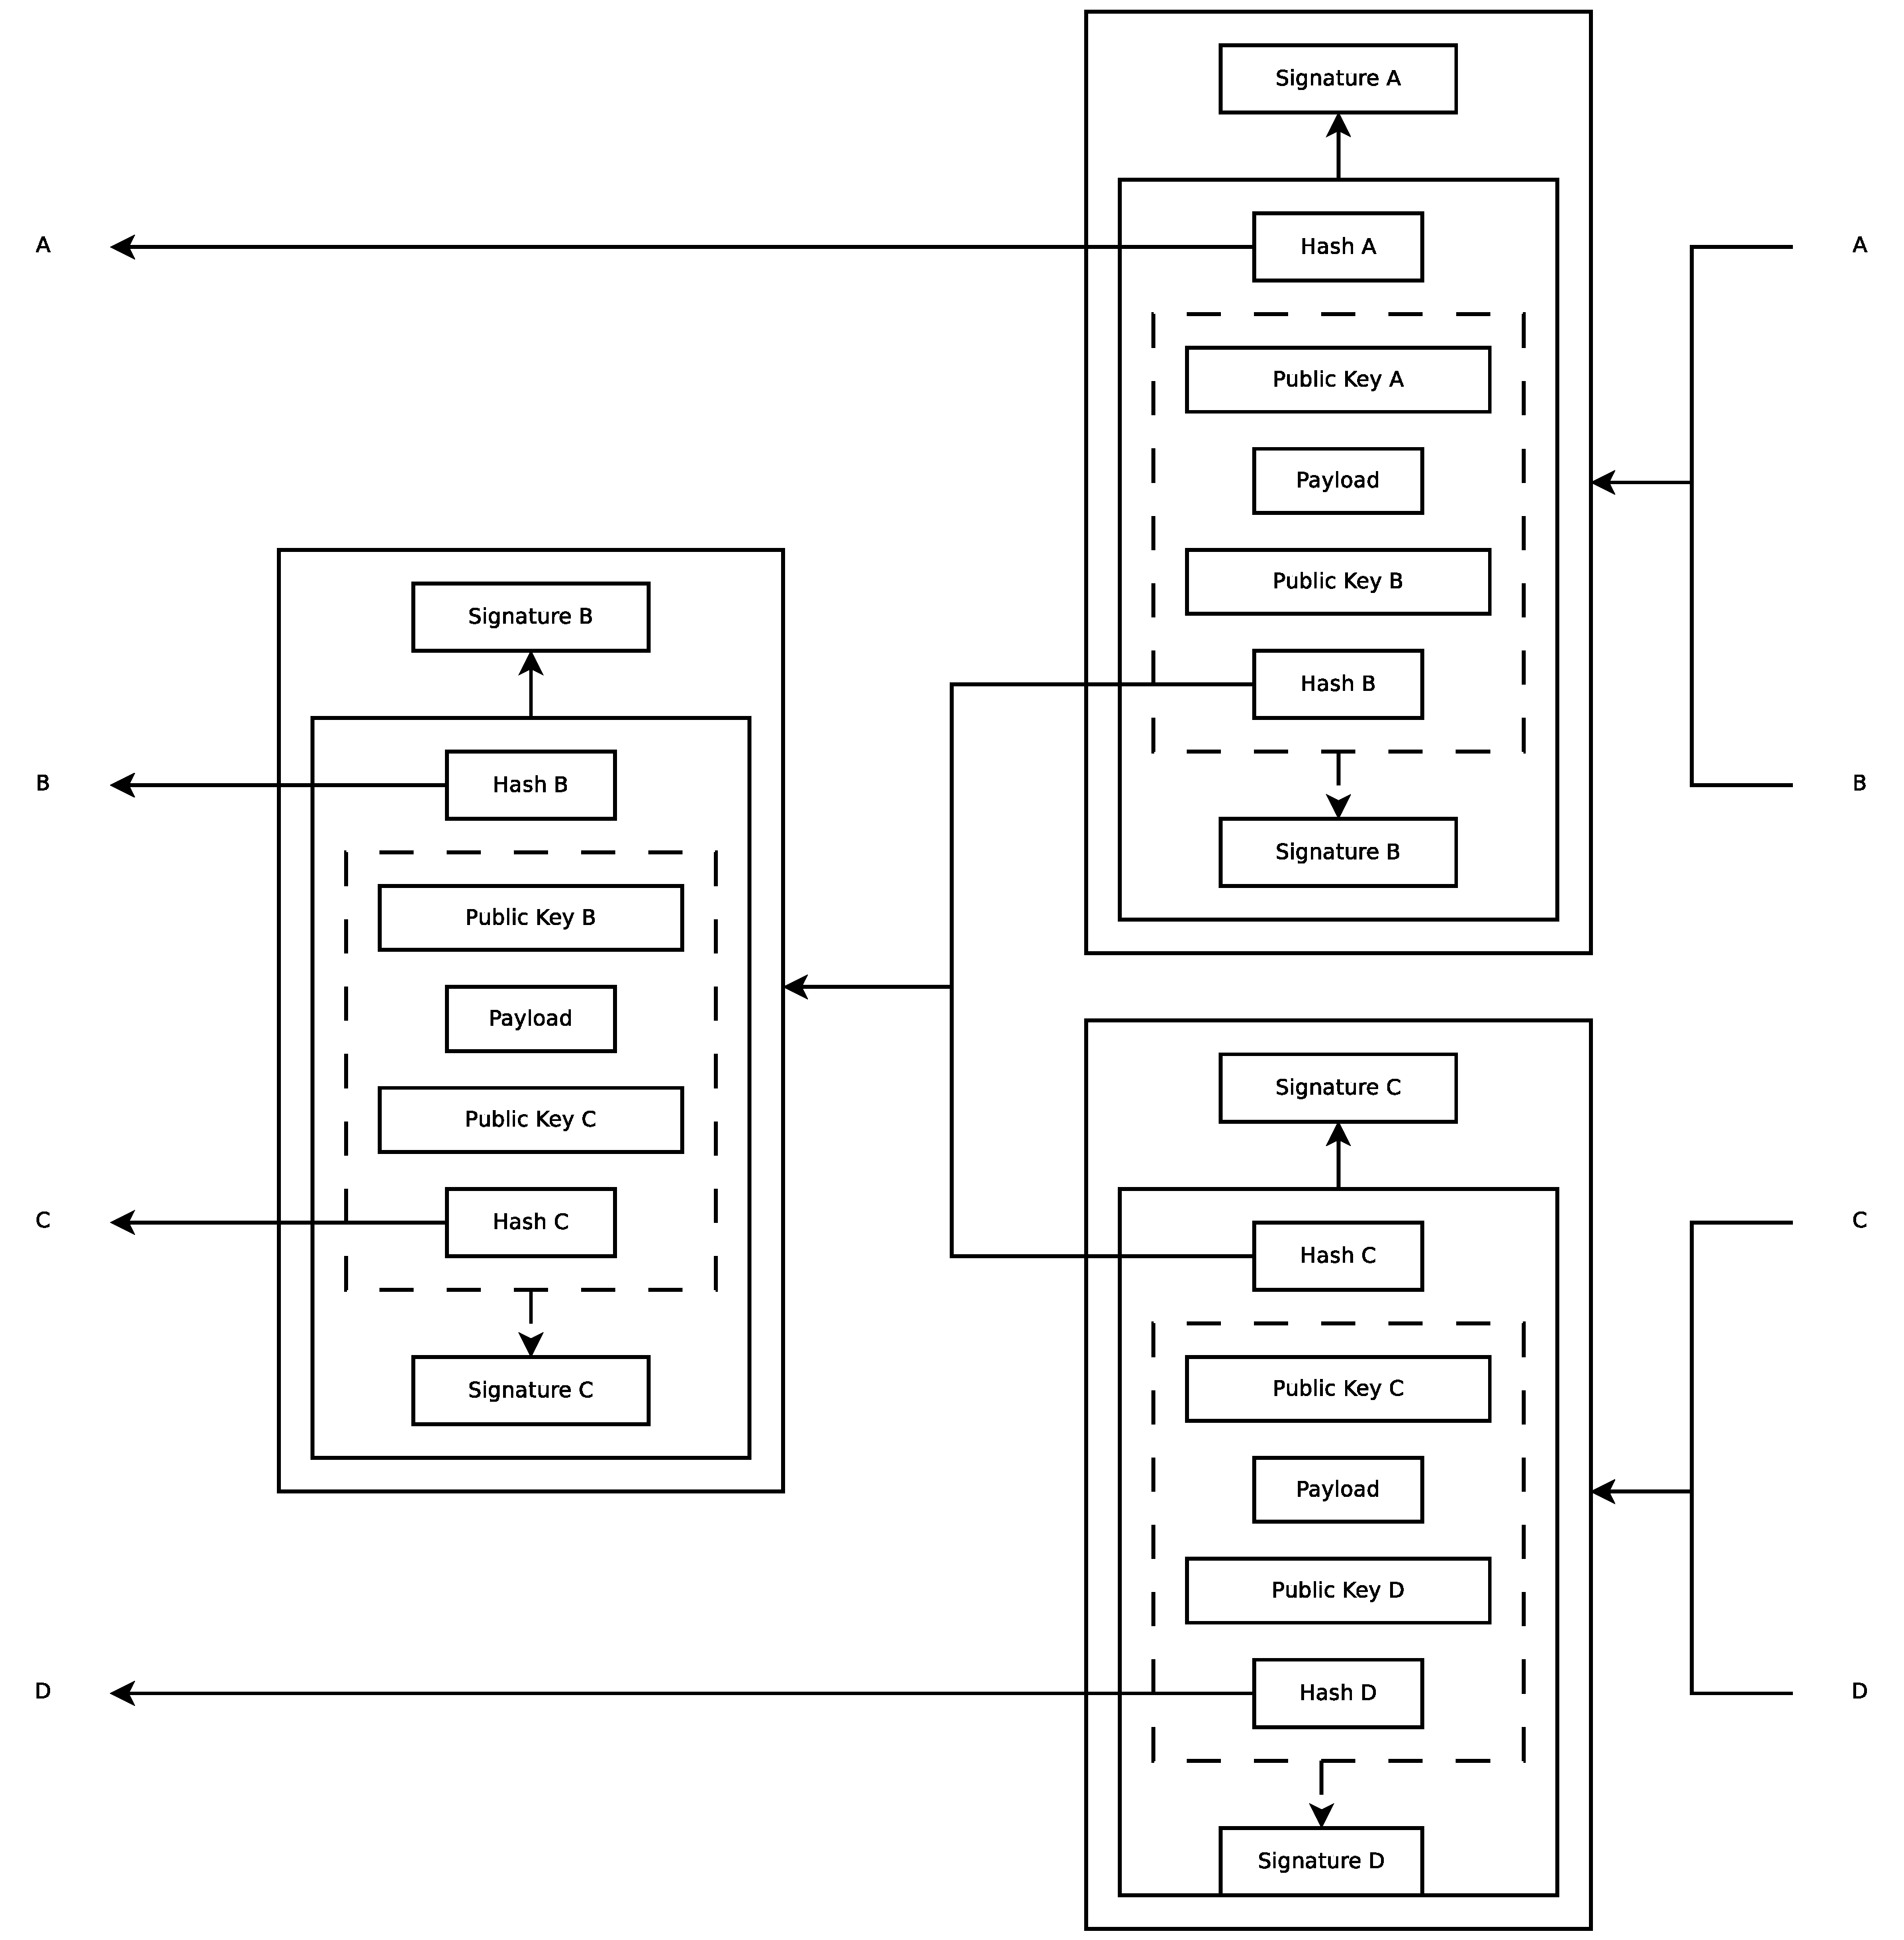
\includegraphics[scale=0.3]{design/figs/chain.eps}}
	\caption{Example of three blocks in the chain.}
	\label{fig:chain-example}
\end{figure}
\subsection{Exchanging signatures}
Two peers in a network will create their blocks together without having to rely on a third party.
Between the peers one is uploading to the other.
The uploader is traditionally called the seeder in BitTorrent and the receiver of this data the downloader~\cite{Cohen-bittorrent}.
The seeder will initiate the block creation.\,
co the seeder can decide how altruistic it wants to be towards the downloader regarding its collaboration.
We will explain how the block creation protocol works.
A sequence diagram can be seen in Figure \ref{fig:exchange-new-sequence}.

\begin{figure}[tpb]
\centering
\subfigure[Sequence diagram for block creation.]{
\centerline{\includegraphics[scale=0.3]{design/figs/exchange_new.eps}}
\label{fig:exchange-new-sequence}
}

\subfigure[Data added by peer A and B for a new block.]{
	\centerline{\includegraphics[scale=0.3]{design/figs/packet_creation.eps}}
\label{fig:packet-creation}
}
\caption{Exchanging data with our cleaner design in Dispersy.}
\label{fig:block-creation-new}
\end{figure}

The seeder, A, will create a packet that will be sent to the downloader, B.
A will add to this packet the data uploaded and downloaded data between the peers
that has not yet been added to the MultiChain.
It will add these amounts to its total uploaded and downloaded data
and add these total amounts aswell to the packet.
Finally, it adds the public keys of both peers and its own hash pointer to the packet.
This packet is signed using its private key and sent to the downloader.
The data that A adds can be seen in Figure \ref{fig:packet-creation}.

B will receive this packet and check if the amounts are correct, if the signature is correct,
and if A has not used the previous hash before.
If this is all correct,
then B will add the amounts of uploaded and downloaded data to its own total amounts.
The data contained in the previous packet, the total amounts of B and the hash of the previous block is
inserted into a new packet.
This packet is signed by the private key of B and sent back to A.
The data that B adds can be seen in Figure \ref{fig:packet-creation}.

Both parties now have the data of the block and can add this to their chain and continue forward.
A does this upon receival of the block.
B does this immediatly after sending the return packet to A.
At this point a new block is created.

\subsubsection{Integrating with Dispersy}
\begin{figure}[!h]
\centering
\subfigure[Sequence diagram for block creation.]{
\centerline{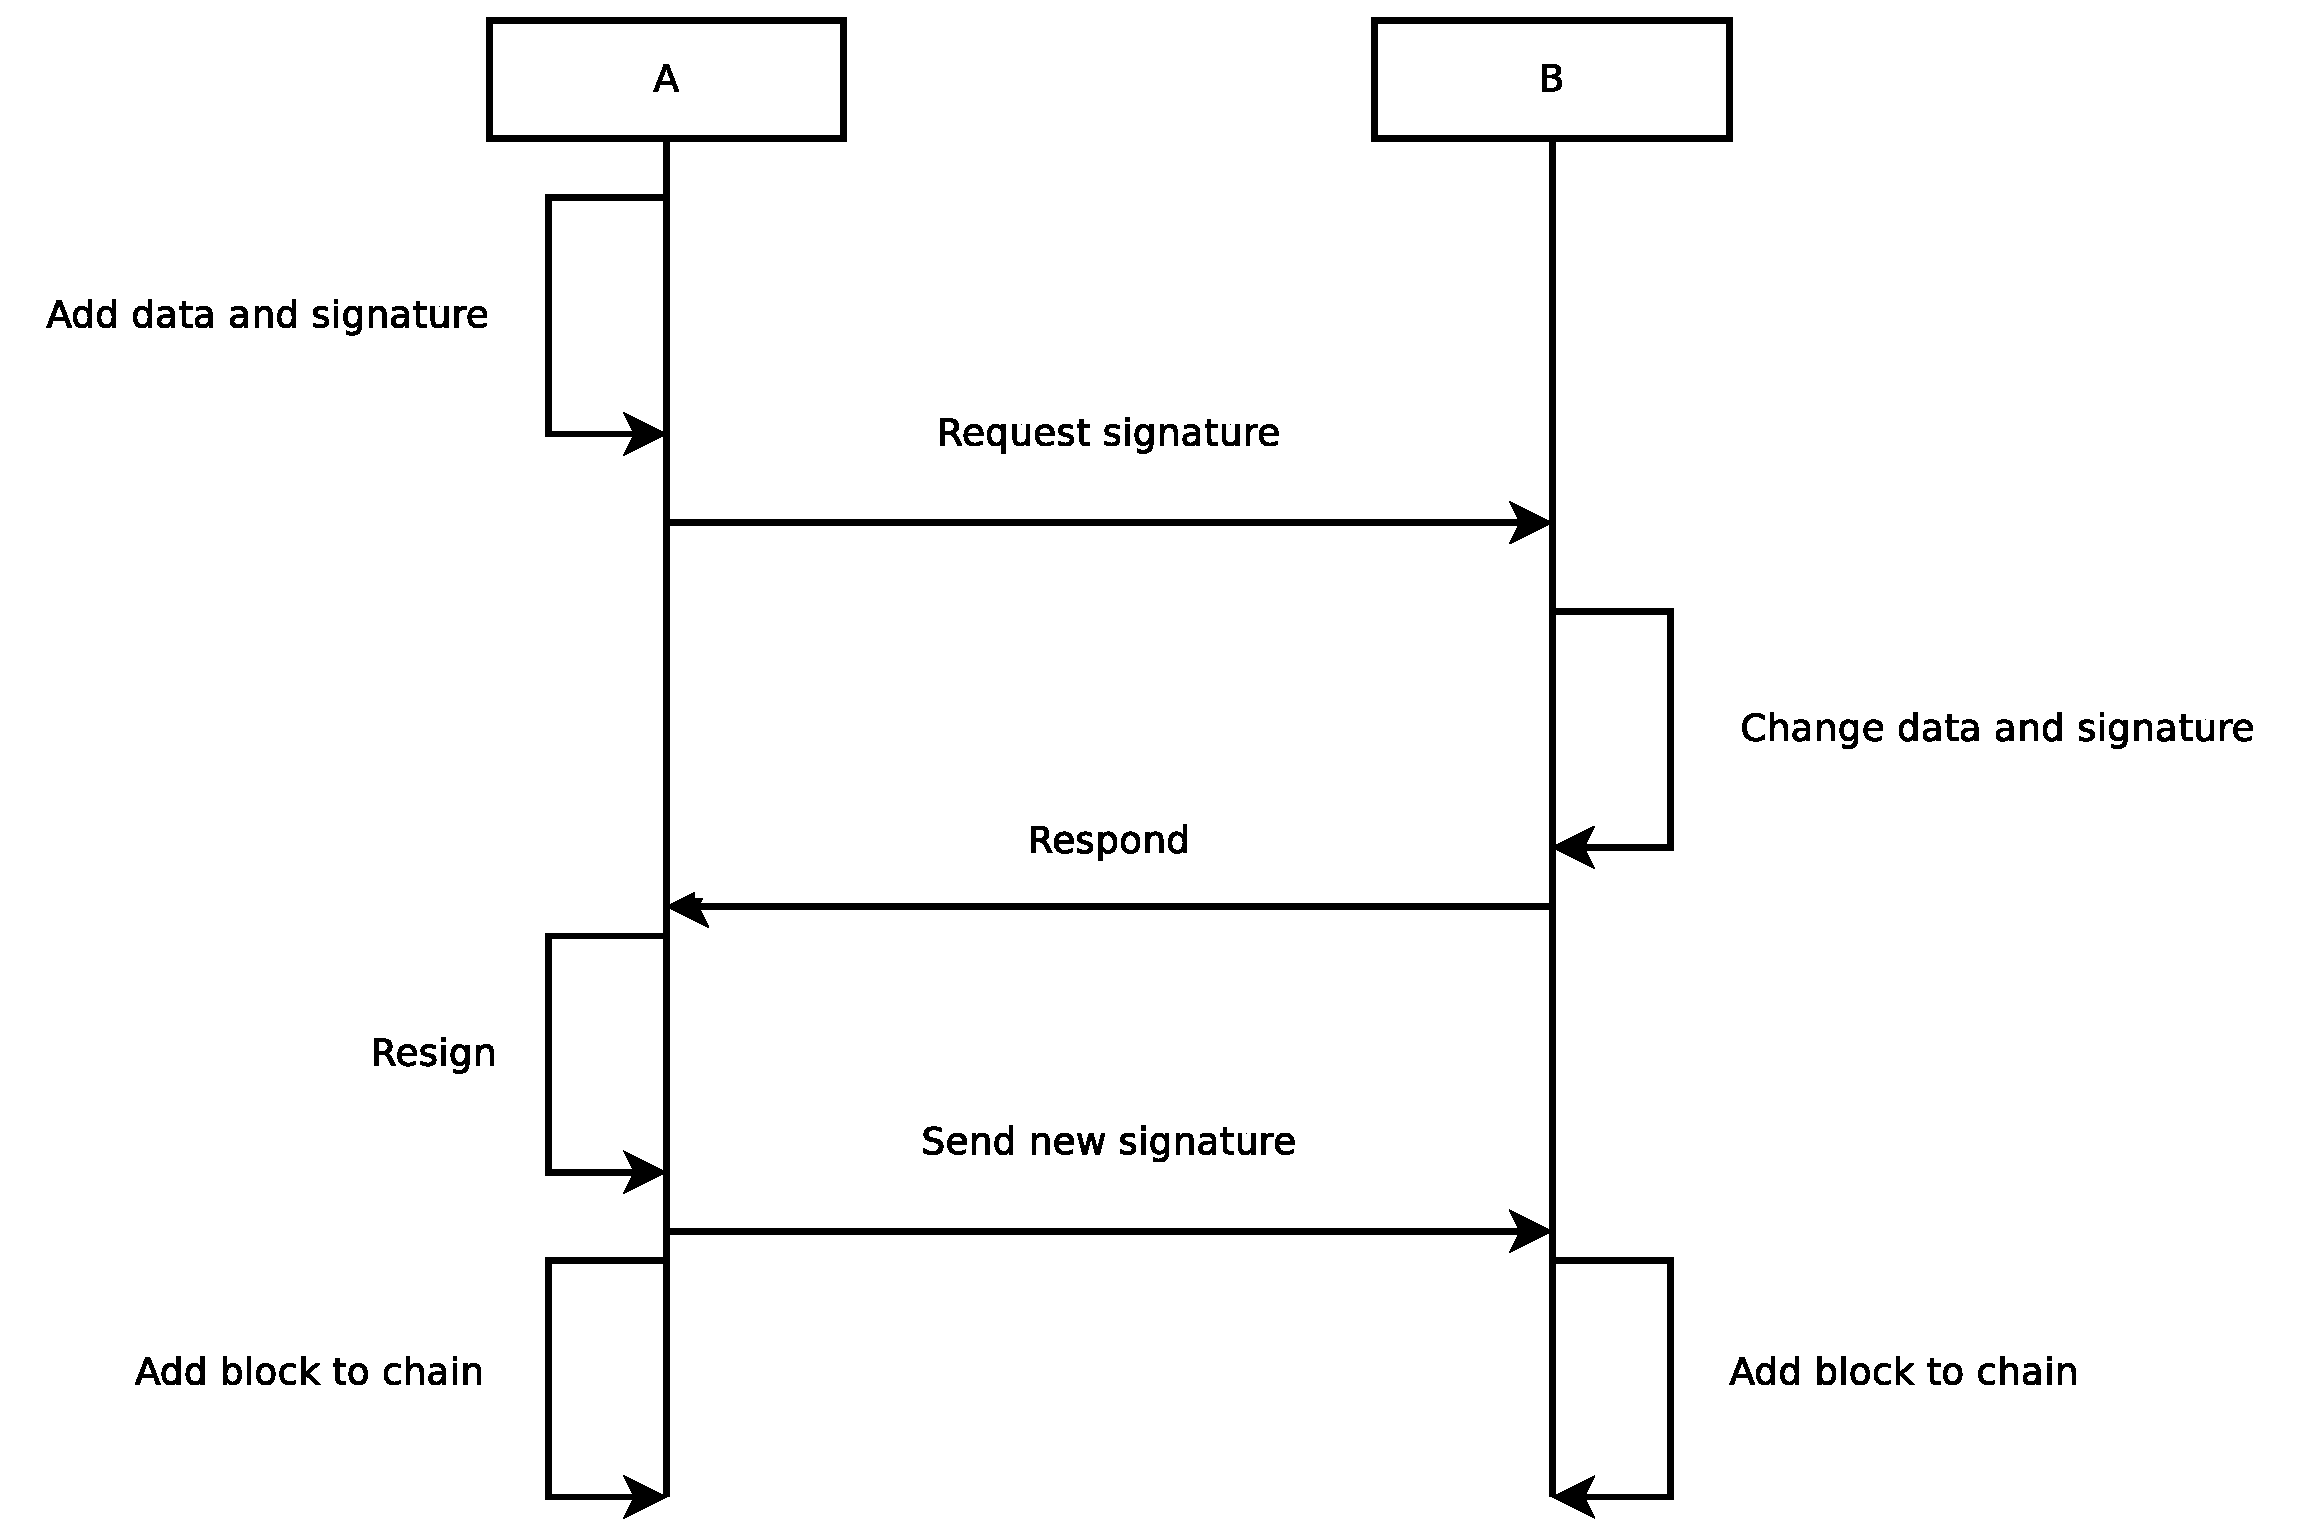
\includegraphics[scale=0.3]{design/figs/exchange_old.eps}}
\label{fig:exchange-old-sequence}
}

\subfigure[Data added by peer A and B for a new block.]{
	\centerline{\includegraphics[scale=0.3]{design/figs/signature_old.eps}}
    \label{fig:payload-signature-old}
}
\caption{Exchanging data for block creation using the old design in Dispersy.}
\label{fig:block-creation-old}
\end{figure}
Within Dispersy functionality was already build to create a message, sign the message
and request multiple nodes to also provide their signature on this message.
This existing functionality could be used by MultiChain to exchange signatures
between A and B for the creation of a new block.

A would initiate a message, insert its data into this message, sign the message, and send this message to B.
The functionality would allow B to accept the message and provide its signature or
modify the message and then provide its signature.
Only B knows the hash of its head node, and the total up and total download metrics.
So B will always modify the message and insert its own data in the message.
But this would invalidate the signature of A,
because the signature of A was also placed on the empty part of the message where the data of B is inserted.
The contents of the message and who signs what can be seen in Figure \ref{fig:payload-signature-old}.

After B returns the message,
A would have to resign the message.
But B also needs this valid signature from A before it can add the block to its own chain.
So A would need to send a third message to with the new, valid signature back to B.
A sequence diagram can be seen in Figure \ref{fig:exchange-old-sequence} of how it would work in Dispersy.
Functionality was added to Dispersy that allows to append data in a signature request.
This allows the full signature exchange to be achieved within two messages.
\section{Atomic operations on the chain}
\label{sect:deadlock}
In a chain, only a single block of a peer is allowed to point to a previous block.
No side branches are allowed.
A peer cannot have multiple blocks belonging to him all pointing to the same previous block.
As this is a potential attack as described in section \ref{sect:branch}.
The chain of a peer can only be moved forward by a single block at any time.
Only after a new block is created, will the new hash available to be used in the next block.

To ensure this happens correctly, the MultiChain community contains mutual exclusive code
that excludes any new operations on the chain if an operation is already pending.
The mutual exclusion is achieved by having to acquire an atomic token to allow to perform an operation on the code.
The MultiChain community will receive incoming signature requests
or requests by other parts of Tribler to send out an outgoing signature request.
The community will decline this request if the token is not available
returns execution to other parts of Tribler.
The token can be unavailable while waiting on another peer in the network to finish responding to a signature request.

When a MultiChain peer has a pending signature request,
then the peer itself will not respond to incoming signature requests from other peers.
These peers themselves will also not respond as they have a pending signature request.
This can create a circular dependency on the availability of the token.
If two peers send a request to each other at the same time, they will wait on each other.
This could result in a deadlock.

MultiChain prevents this deadlock to occur by allowing a transaction to fail
as explained in section \ref{des:halfsigned}.
If MultiChain gets into this potential deadlock one of the peers will eventually time out of their own signature request
and process the incoming request resolving the circular dependency.
The deadlock is recovered and both peers can continue operation.
This situation has occured during experimentation and it is explained in section \ref{sect:deadlock-exp}.
It is shown that MultiChain correctly recovers the potential deadlock.
A potential attack vector is explained in \ref{sect:denial}


\section{Block persistence}
The blocks in the chain have to be persisted to be usable over a prolonged time.
A persistence layer is added to the MultiChain community
that provides all functionality to persist blocks and query blocks.
This layer extends and uses functionality of the Database class in Dispersy.
An overview of the layering in the software architecture can be seen in Figure \ref{fig:persistence-layer}.

\begin{figure}
	\centerline{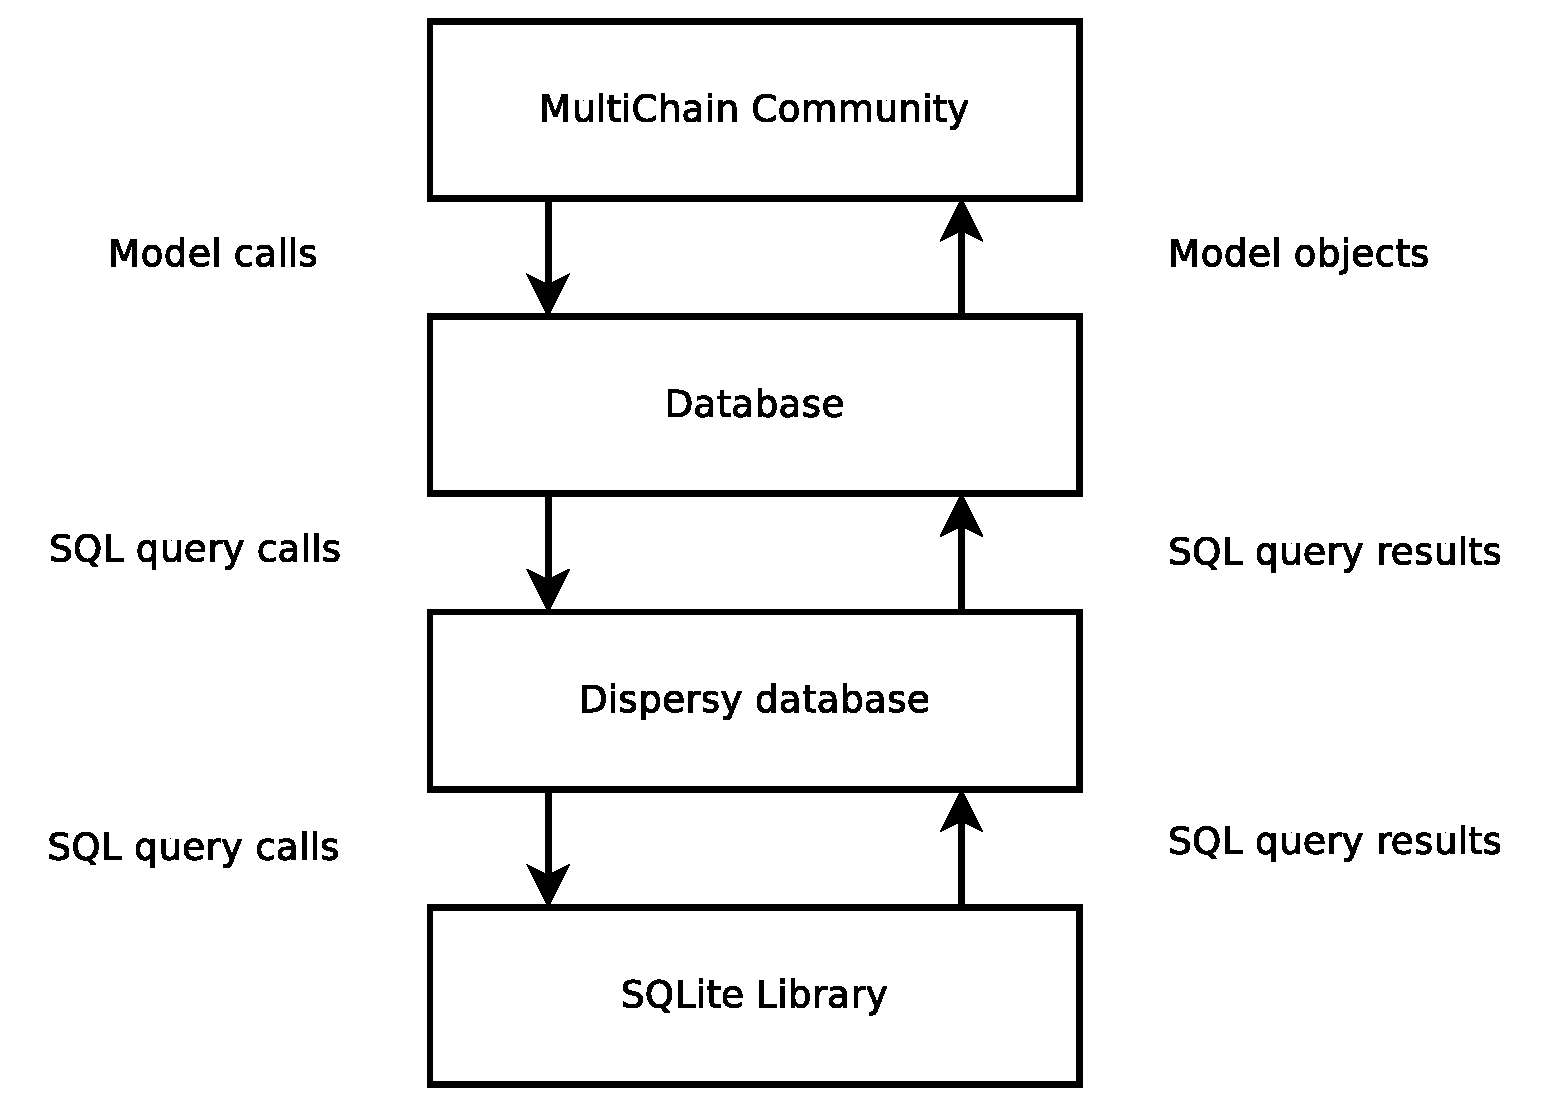
\includegraphics[scale=0.3]{design/figs/persistence-layer.eps}}
	\caption{Persistence layering in the software architecture}
	\label{fig:persistence-layer}
\end{figure}

The MultiChain Community calls functions in the persistence layer that have implicit knowledge about the model.
The Persistence layer formats SQL queries and passes these to the Dispersy layer.
The Dispersy layer performs several sanitation checks and passes these queries to the SQLite Library.
The SQLite Library and Dispersy layer both return the result of the SQL query.
These results are transformed by the Persistence layer into objects of the model usable by the MultiChain Community.

The only information that is saved are blocks.
The information all fits within one table.
A single block is saved as a single record called a row in a relation database.
Every attribute of a block is a single column in the row.
All attributes are saved directly into the database,
except for the public keys.
These public keys are hashed and these hashes are used as an identifier, called mid, in Dispersy.
The public keys are already saved in the Dispersy database.
When a block is retrieved from the database the public key is retrieved from Dispersy using the mid.

Every attribute is queryable in the database.
A public key can be converted to mid and is searched this way.
Every attribute is queryable to make the system  extensible
and usable when the next incremental steps are implemented.
It is presently unknown what information precisly will be needed,
so every information is now made available for the future.

\subsection{Dispersy database}
Dispersy keeps track of information on its own.
A record is kept of any message that can be retrieved using a message id.
The message is saved in a converted format and will be decoded when the message is retrieved.

Instead of storing information in a separate database,
the information could have been retrieved from the Dispersy database.
But the Dispersy database is not queryable.
All the information is stored in a converted format
that prevents queries to search the message for its contents.
For this reason, the dispersy database is not used and a separate database is used.

A future, possible improvement to Dispersy would be to save messages queryable in its database.
This would eliminate the current need for separate databases that contain aggregrated information.
The information is stored in two places within Tribler and this could be eliminated.
It would reduce the disk footprint and the amount of read/write transactions
as only one database would have to be maintained.
The I/O ineractions are a problem according to Tribler maintainers.

\section{Integration with Tribler}
The MultiChain community can be run standalone,
but its main use is to integrate with Tribler and track up and download for torrents.
It will replace the current reputation system Bartercast in the future.

For integration a scheduler is implemented between the MultiChain community
and the community that handles the anonymous download.
For additional detail on the anonymous download communities see \cite{Plak-anonymous}\cite{ruigrok-anonymous}.
The scheduler tracks session up and download amounts and schedules a block to be created,
when the amount of uploaded bytes is above a certain threshold.
The scheduler currently only tracks traffic of anonymous downloads.
Bartercast is not yet removed and
currently MultiChain runs together with Bartercast untill MultiChain fully replaces Bartercast.

The scheduler should be expanded in the future to schedule blocks in a more sophisticated way.
The functionality of the scheduler is very limited and is missing basic functionality.
The most important improvement that should be introduced is the punishment of not signing blocks.
Currently, nodes can deny to have their behaviour tracked.
The next improvement is to actually determine the level of cooperation a node receives based upon their previous behaviour.
The actual decision making based upon past behaviour is not part of the thesis.
\section{Crawler}
A crawler was implemented that visits other nodes and request the full chain of that node.
The crawler was used for the experiments and
is a first step in a more sophisticated crawler that will help to solve the known vulnerabilities.
These vulnerabilities will be described in chapter \ref{problems}.

\subsection{Recursively request blocks}
Dispersy provides a list of other nodes that were recently found
and can report when the node itself is found by an other node.
Both are sources of destinations nodes that the crawler will visit
and request the chain from.

The crawler will first request from a node the block with sequence number $-1$.
This denotes that he wants the latest block in his chain.
The node returns this block to the crawler.
The crawler will persist the block if it is not yet know.

The newly retrieved block is chained to two blocks with the previous hashes.
The crawler will check if these blocks are present in the database.
If any block is not present,
then the crawler will request that particulair block if the node is known in Dispersy.
If the node is not known, the block is ignored.
This is done recursively untill the crawler reaches the genesis block of the chain.
In this fashion a breadth first search is implemented for any unknown block
that is chained in chronologically before the latest block.

\begin{figure}
	\centerline{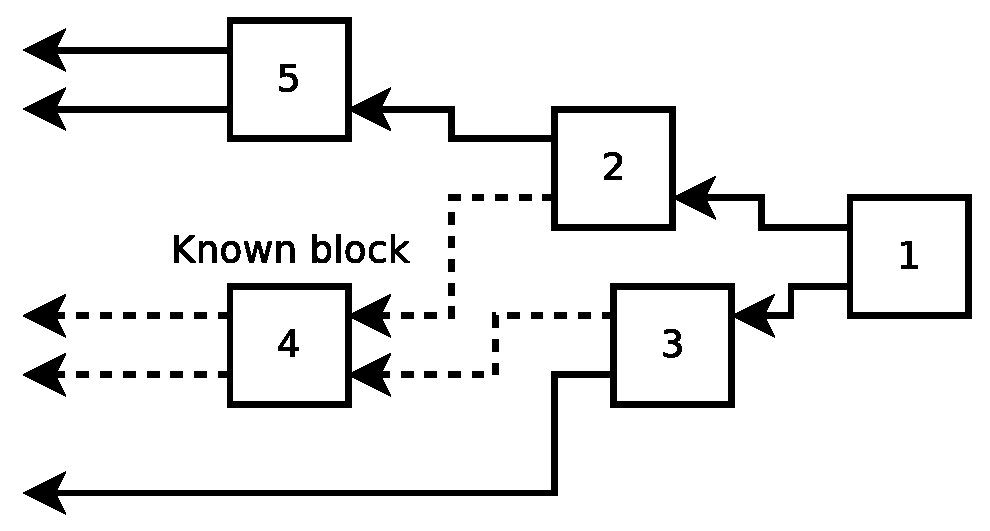
\includegraphics[scale=0.3]{design/figs/crawler.eps}}
	\caption{Example of the crawler looking for unknown blocks.}
	\label{fig:crawler-example}
\end{figure}

An example can be seen in Figure \ref{fig:crawler-example}.
In this example the line arrows denote paths that the crawler follows
and dotted lines are paths that the crawler ignores.
Block 4 is already known by the crawler.
Block 1 is retrieved by the crawler and the crawler sees hash links to block 2 and 3.
These are retrieved and the block finds links to block 4 and 5.
Because block 4 is already known, block 4 is ignored.
Only block 5 is retrieved.
The crawler follows the links further outside the displayed example.

\subsection{Improvements}
The crawler is a first, simple step towards a more sophisticated crawler.
Tribler has implemented already more sophisticated crawlers for Bartercast
and these techniques can be reused for the MultiChain crawler.
For example bloom filters can be used in conjunction with the knowledge
that every record is a part of the chain to quickly request multiple blocks\cite{broder-bloomfilter}\cite{logiotatidis-splash}.
Blocks could also be send in a more efficient way by sending multiple blocks per message.
Lastly an obvious improvement is to also crawl and retrieve blocks from other nodes present in a node.
This is currently not yet implemented.



\section{Anonymity}
Tribler has made an effort in providing a way for users to download anonymously\cite{Plak-anonymous}\cite{ruigrok-anonymous}.
There is anonymity in the contents of what is downloaded, not in how much is downloaded.
MultiChain obviously cannot break this anonymity to be usuable for anonymous downloads.
The introduction of anonymity increases the necessity of a good reputation system as more data has to be transferred.

MultiChain only interacts with peers that are directly downloaded from or uploaded to.
With these peers blocks are created and transferred.
So anonymity is not broken by MultiChain.
An attacker could already analyse network traffic between these peers
and conclude they are downloading and uploading to each other.
But Tribler does not guarantee anonymity for this.
So MultiChain does not break anonymity with its interactions with peers.

A block only transcribe the amount of data that has been transferred between peers.
The content of the actual data is not transcribed.
The block also does not leak information of how big a single, individual transfer is between peers.
The amounts are aggregrated over all transfers.
The blocks also does not break the anonymity.
Network analysis can already measure the total amount of data transferred.
So the design and implementation of MultiChain does not break anonymity already guaranteed by Tribler.

But MultiChain does make network analysis easier as measurement points between every node do not have to be introduced.
The chain of every node can be requested.k
The chain contains the data of every transaction of a peer and can be used to analyse the network.

%Experimentation
\chapter{Experimentation}

In this chapter multiple graphs are depicted.
These graphs are generated by reading every database of every node.
The blocks are depicted as nodes and the previous hash pointers are edges in the graph.
The nodes have added colouring to indicate extra meaning.
Green nodes are a first block in a MultiChain of a peer,
and as such have no inbound arrows.
Blue nodes are a sequential block between the same previous peers,
therefore they do not have two inbound arrows.
Red nodes are half-signed blocks,
and therefore only have one inbound and one outbound arrow.

Some experiments were also run multiple times because Dispersy does not always connect to every peer.
At the start of the experiment the peers are forced to be introduced,
but this does not always succeed.
This is a problem in discoverability and has been experienced by previous work aswell\cite{ruigrok-anonymous}.
This also happens when downloading a torrent in the real world.
The final version is chosen when Dispersy did connect all the peers.

\section{Software engineering tests}
MultiChain is tested in several ways to verify it is correctly working
following standard software engineering practices.
These tests work similair to other tests used to test Tribler.

Tribler uses Python unit tests  to validate small components of code.
The tests can be run locally and
are automatically run on a Jenkins build server\cite{jenkins}\cite{jenkins-tribler}.
Unit tests are added to increase stability of MultiChain.
Tribler does prove to be hard to test using unit tests.
This is due to high coupling of code within Tribler.
But mocking of classes helped in testing difficult to test code.
The separate unit tests for the conversion, payload and database were the first of it types inside Tribler.
\todo{Update the table}
An overview of the coverage can be seen in Table \ref{tab:tests}

\begin{table}
\centering
\begin{tabular}{l|ll|ll}
Filename   & LOC & \%    & Conditionals & \%    \\ \hline
Community  & 187 & 86\%  & 37           & 62\%  \\
Conversion & 60  & 95\%  & 6            & 50\%  \\
Database   & 113 & 87\%  & 10           & 50\%  \\
Payload    & 89  & 100\% & 2            & 100\% \\ \hline
Total      & 672 &       & 47           &
\end{tabular}
\caption{Unit tests coverage of MultiChain.}
\label{tab:tests}
\end{table}

Next to that, Tribler uses a separated developed test runner Gumby.
Gumby can start multiple instances of Tribler and follow test scenario's.
Gumby can be used to perform system tests and experiments.
These system tests have to be manually validated.
Several scenario's have been written to validate MultiChain.
These run MultiChain either in a standalone version or integrated into the TunnelCommunity.

One of these scenario's can be found in Listing \ref{fig:exp-gumby-scenario}
In this example basic block creation is tested.
Normal situations are tested,
but also situations where the signature requests are answered late
and other requests arrive at the requesting peer at the same time.
Additionally, signature requests are controlled to not be answered at all.
During the whole test the crawler is active and scrapes the network for unknown blocks.
The notation in the scenario is the time an action has to be taken place,
the action that has to be taken, and by who if necessary.

\begin{figure}
\begin{FVerbatim}[fontsize=\small]
@0:0 set_master_member 3081a7301006072a8648ce ... 2b51
@0:0 set_community_class MultiChainNoResponseCommunity {4}
@0:0 set_community_class MultiChainDelayCommunity {5}
@0:0 set_community_class MultiChainCommunityCrawler {6}
@0:0 set_community_class {6}
@0:0 start_dispersy
@0:1 online
@0:5 reset_dispersy_statistics
@0:10 annotate start-experiment-1-peer
@0:15 introduce_candidates
@0:80 request_signature 2 {1}
@0:84 request_signature 1 {2}
@0:94 request_signature 4 {1}
@0:95 request_signature 1 {3}
@0:104 request_signature 5 {1}
@0:106 request_block 1 5 {6}
@0:110 close
@0:111 stop_dispersy
@0:112 stop
\end{FVerbatim}
    \caption{One fo the gumby test scenarios}
    \label{fig:exp-gumby-scenario}
\end{figure}

\section{Tracking download and upload amounts}
\section{Single block creation}
In this experiment we try to create a block between two nodes.
This experiment validates the MultiChain to be able to correctly create a block between nodes in normal circumstances.
The experiment is locally run using gumby with all nodes running on a single computer.
Only two instances of MultiChain communities are started and between these two communities a block is created.
The logging of the both nodes is captured and recorded to verify the results of the experiment.

The output of the logging can be seen in figure \ref{fig:singleblockexperiment}.
First node 1 sends a signature request to node 2.
This message is received and a block is persisted.
The hash of the block is displayed in the output.
The block is sent back as a signature response to node 1.
The block is saved by node 1 and has the same hash as shown in the output.
So the block between node 1 and node 2 is the same and a block was succesfully created.
The output also shows behaviour of MultiChain
to correctly exclude any other execution from entering mutual exclusive code.
The lines related to the mutual exclusion are prepended by "Chain Excl".
The nodes check if it is possible to enter the mutual exclusive part and correctly acquires
and releases the mutual exclusion token.


\begin{figure}
    \begin{SaveVerbatim}{VerbCode}
OUT: 1: Requesting Signature for candidate: 2
OUT: 1: Chain Excl: signature request: False
OUT: 1: Chain Excl: acquired, sending signature request.
OUT: 1: Sending signature request.
OUT: 2: Received signature request.
OUT: 2: Chain Excl: process request: False
OUT: 2: Chain Excl: acquired to process request.
OUT: 2: Persisting sr: 2F7bTMxyJU7hZkvaBimT2bYm4bY=
OUT: 2: Chain Excl: released after processing request.
OUT: 2: Sending signature response.
OUT: 1: Signature response received. Modified: True
OUT: 1: Valid 1 signature response(s) received.
OUT: 1: Persisting sr: 2F7bTMxyJU7hZkvaBimT2bYm4bY=
OUT: 1: Chain Excl: released after signature response.
    \end{SaveVerbatim}
    \setlength{\fboxsep}{5mm}
    \fbox{\BUseVerbatim{VerbCode}}
    \caption{Output of single block creation experiment}~\label{fig:singleblockexperiment}
\end{figure}
\subsection{Chaining blocks}
The next experiment we experiment with MultiChain creating a chain of blocks between two peers.
The experiment is run using gumby with all peers running on a single computer.
We try to create 10 subsequent blocks mimicking a download of 10MB with a speed of 1000 KB/s.
Every second these amounts are indicated to have been transferred to the schedulers of every peer.
The scheduler waits for 1MB uploaded to another peer before scheduling a block.

The result of the experiment can be seen in the graph in Figure \ref{fig:chain-experiment-graph}.
In this graph it can be clearly seen that MultiChain is succesful in creating a chain of 10 blocks.

\begin{figure}[!h]
	\centerline{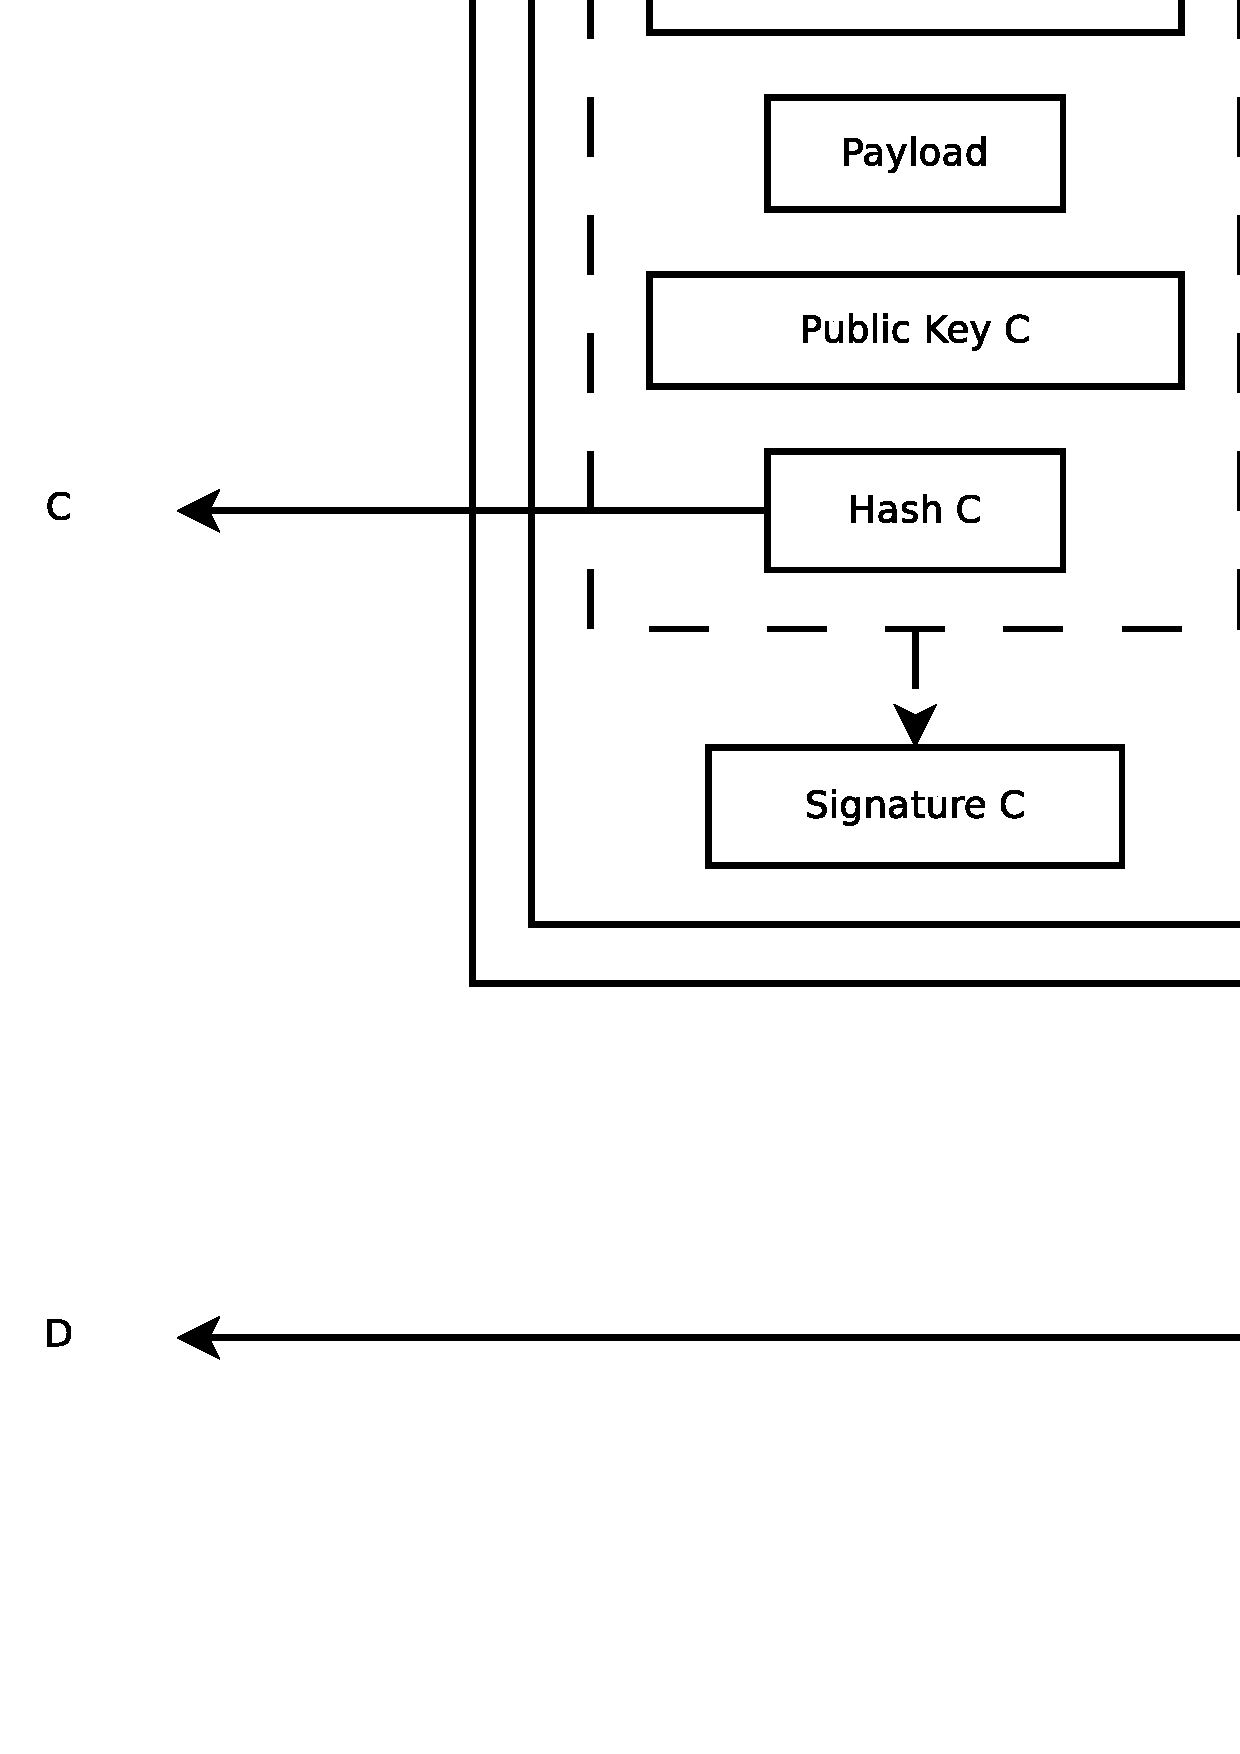
\includegraphics[scale=0.20]{experimentation/chain/chain.png}}
	\caption{MultiChain chain graph of a single download of 10 MB.}
	\label{fig:chain-experiment-graph}
\end{figure}

The amounts stored in each blocks are plotted in Figure \ref{fig:chain-experiment-amounts}.
Every datapoint is a block in the chain of a peer and is the the total amount stored in that block..
These datapoints are connected by a dotted line representing the link between these blocks.
These plots show that MultiChain correctly tracks the download of 10MB.
The slope of the figure corresponds with the speed of the download.

\begin{figure}
\centering
\subfigure[Total download amount.]{
\centerline{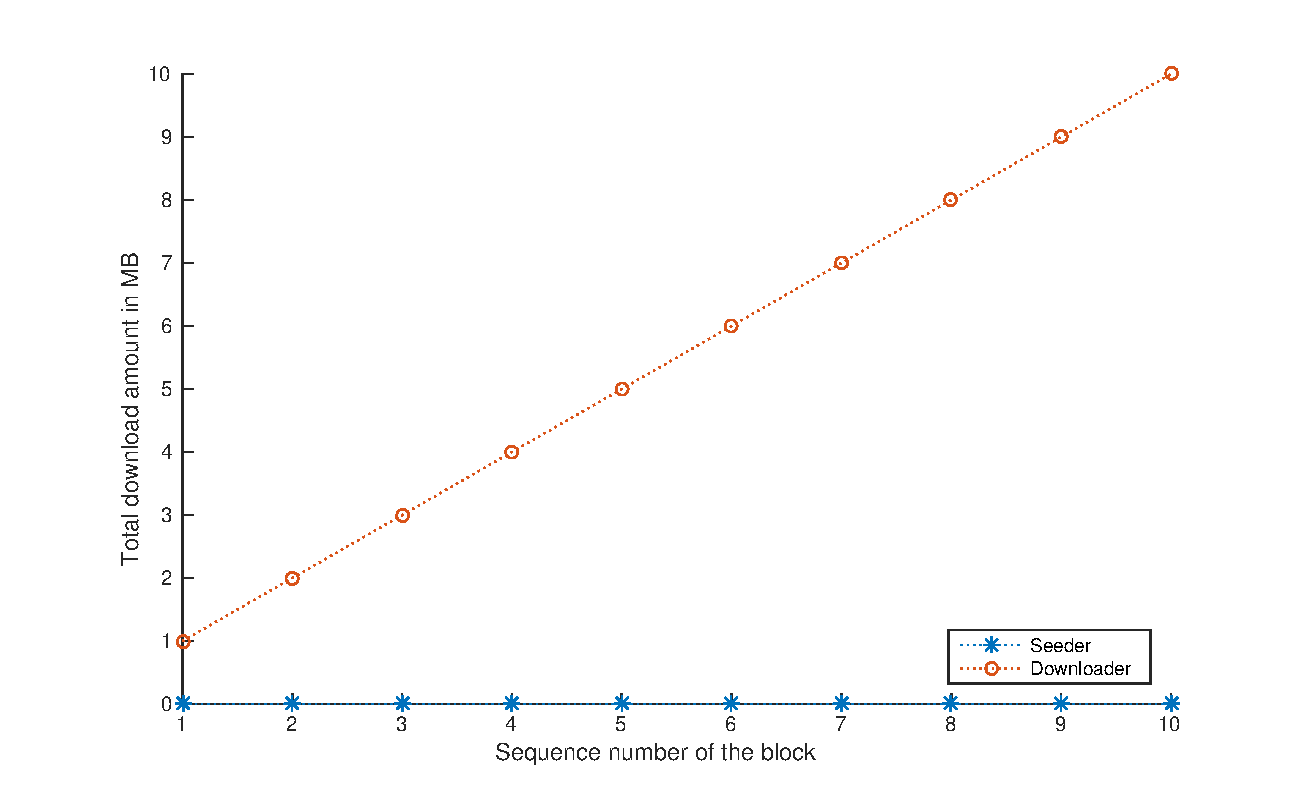
\includegraphics[scale=0.5]{experimentation/chain/chain-down.eps}}
\label{fig:chain-experiment-down}
}
\subfigure[Total upload amount.]{
\centerline{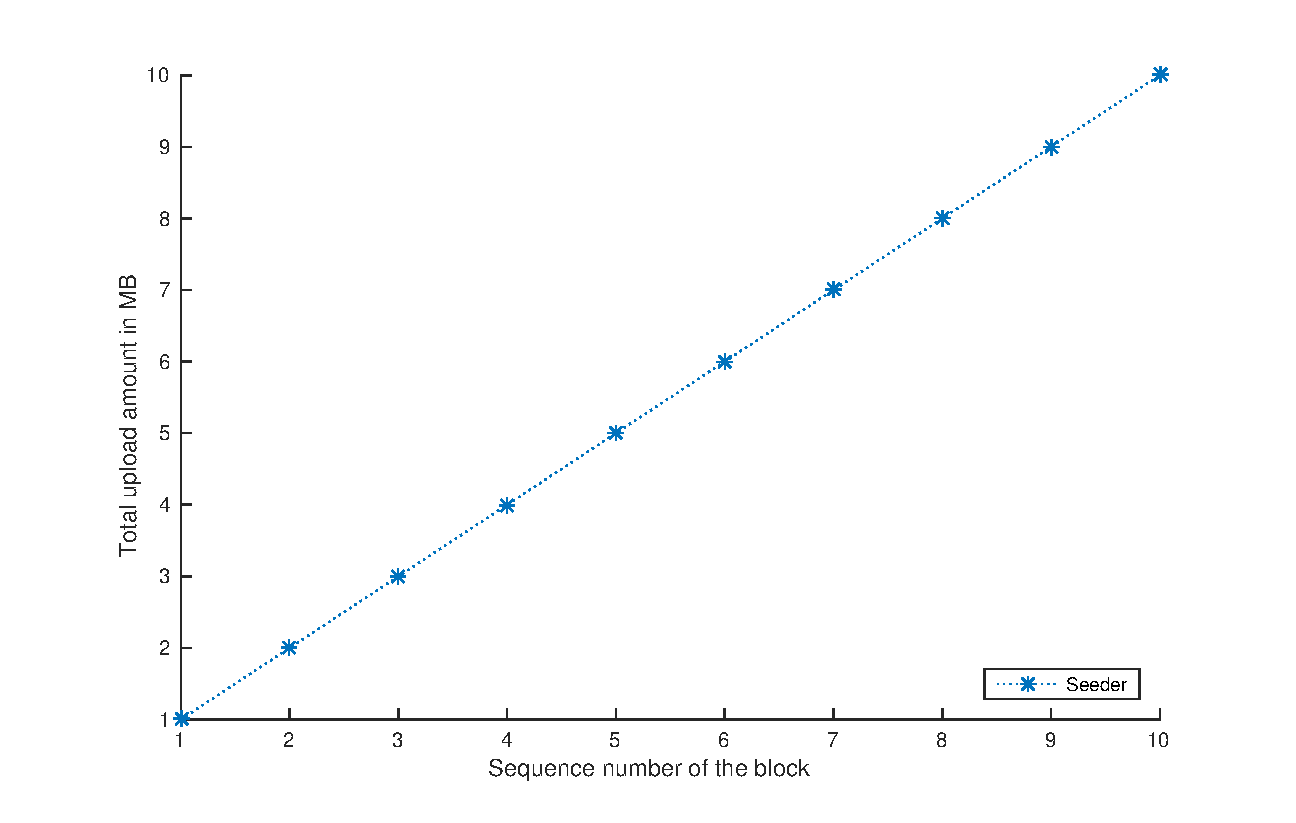
\includegraphics[scale=0.5]{experimentation/chain/chain-up.eps}}
\label{fig:chain-experiment-up}
}
\caption{Download and upload amounts when creating a chain of 10 blocks.}
\label{fig:chain-experiment-amounts}
\end{figure}

\subsection{Tracking downloads with different speeds}
In this experiment we measure if MultiChain can correctly track the upload and download amounts
between two peers with different speeds.
In the scenario a file of 100 MB is downloaded at different speeds,
respectively 500 KB/s, 750 KB/s, 1000 KB/s, 1250 KB/s, 2000 KB/s, and 3000 KB/s.
The maximum speed of anonymous download was measured in experiments to be 1150 KB/s\cite{ruigrok-anonymous}.
The scheduler waits for 1MB uploaded to another peer before scheduling a block.
The upload and download of the file is done by different pairs of seeders and leechers.
Every second these amounts are indicated to have been transferred to the schedulers of every peer.

\begin{figure}
\centering
\subfigure[Total download amount.]{
\centerline{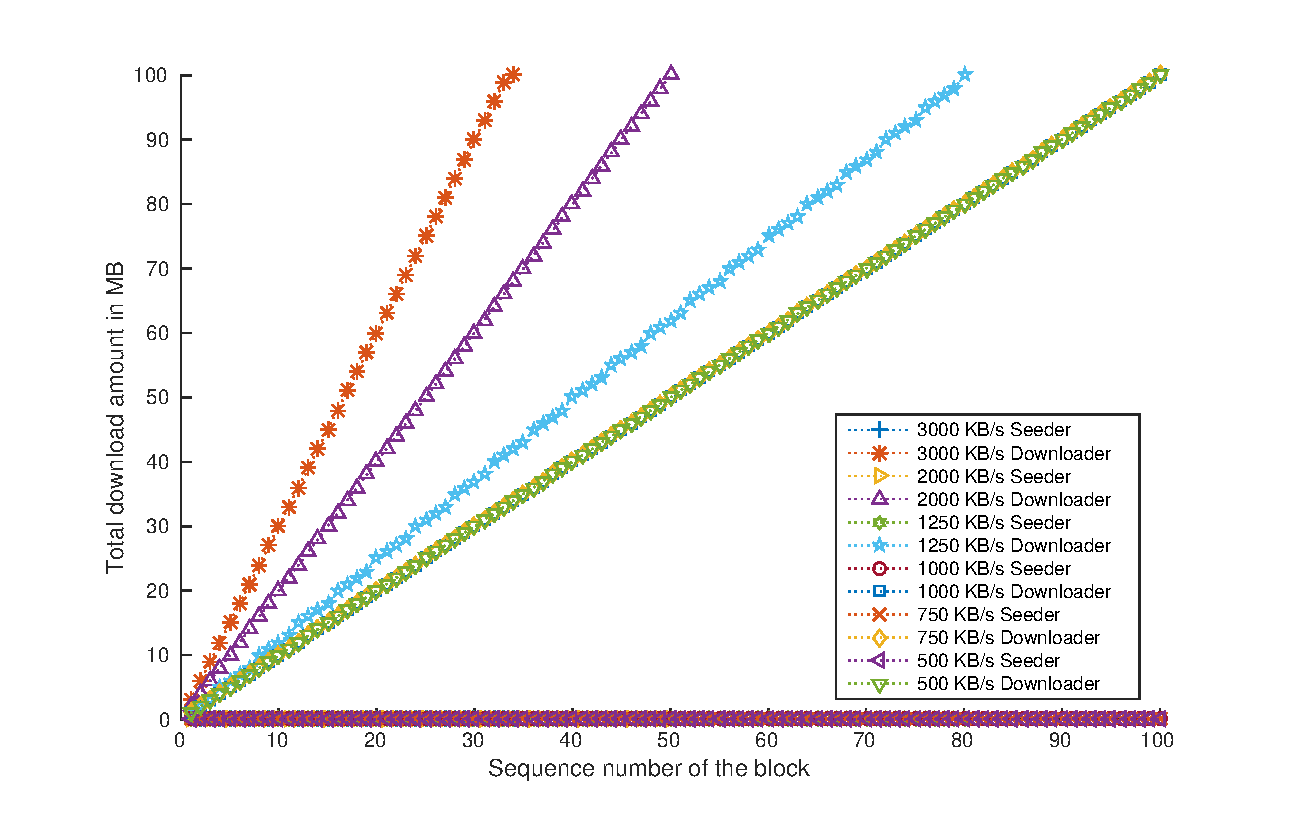
\includegraphics[scale=0.5]{experimentation/speeds/synthetic-simple-down.eps}}
\label{fig:synthetic-simple-down}
}
\subfigure[Total upload amount.]{
\centerline{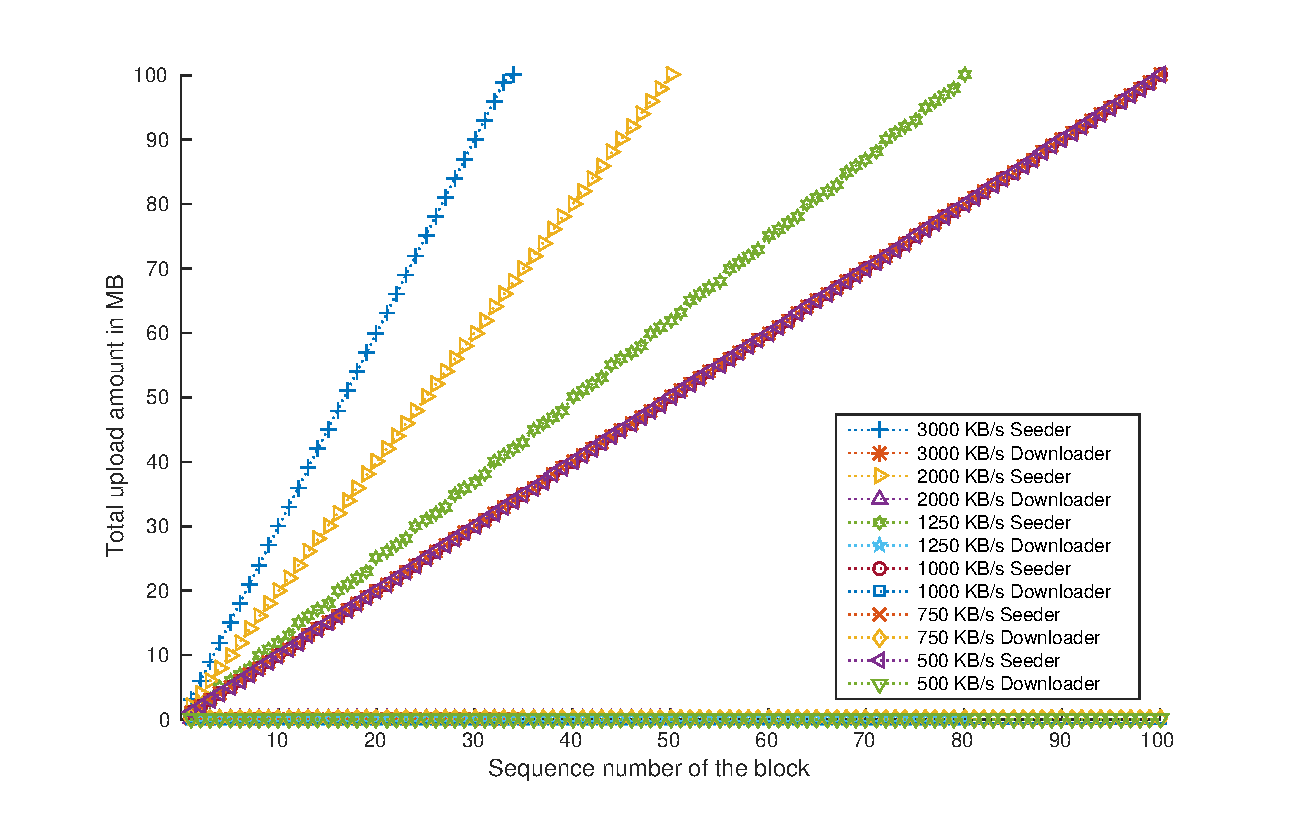
\includegraphics[scale=0.5]{experimentation/speeds/synthetic-simple-up.eps}}
\label{fig:synthetic-simple-up}
}
\caption{Download and upload amounts when tracking downloads at different speeds.}
\label{fig:synthetic-simple-amounts}
\end{figure}

The total download and upload amounts of every peer is plotted in Figure \ref{fig:synthetic-simple-amounts}.
These amounts are plotted in the same way as the previous experiment.
The plots show that MultiChain is able to correctly track the download and upload amounts without a problem.
There are no hitches in the figures and the amounts go up in fixed increments corresponding to the different speeds.
This means that MultiChain is fast enough to correctly track the amounts.

The download speeds below the threshold of 1000 MB of the scheduler
are not distinguishable from the download at the threshold speed.
This is because the scheduler waits until the threshold is reached before initiating the block.
The amount is tracked in the same amount of blocks,
but the total time of the experiment is longer for these experiments.
If the speed goes above the threshold, then this is reflected in the figure.

The graph in Figure \ref{fig:synthetic-simple-graph} shows the graph of the blocks created by the experiment.
The graph is disconnected, because the different pairs of seeders and leechers did not interact with each other.
So no block that would connect their chains is created,
This leaves the graph disconnected.

\begin{figure}
	\centerline{\includegraphics[scale=0.06]{experimentation/speeds/synthetic.png}}
	\caption{Disconnected chain graph of tracking downloads at different speeds.}
	\label{fig:synthetic-simple-graph}
\end{figure}

This experiment was run several times before the final version in this report was run.
Earlier versions of the experiment resulted in two bugfix and two improvements:
the ability of the scheduler to create a block at the end of a download.
\subsection{Synthetic anonymous download}
In an anonymous download scenario the data is downloaded through multiple hops.
A seeder uploads data to the first hop.
This hop relays the data to the second hop.
The second hop sends the data to its destination at the leecher.
This can be seen as sequence of peers and is illustrated in Figure \ref{fig:seeder-hops-leecher}.
More hops can be added to better safegaurd the anonymity of the download.

\begin{figure}
	\centerline{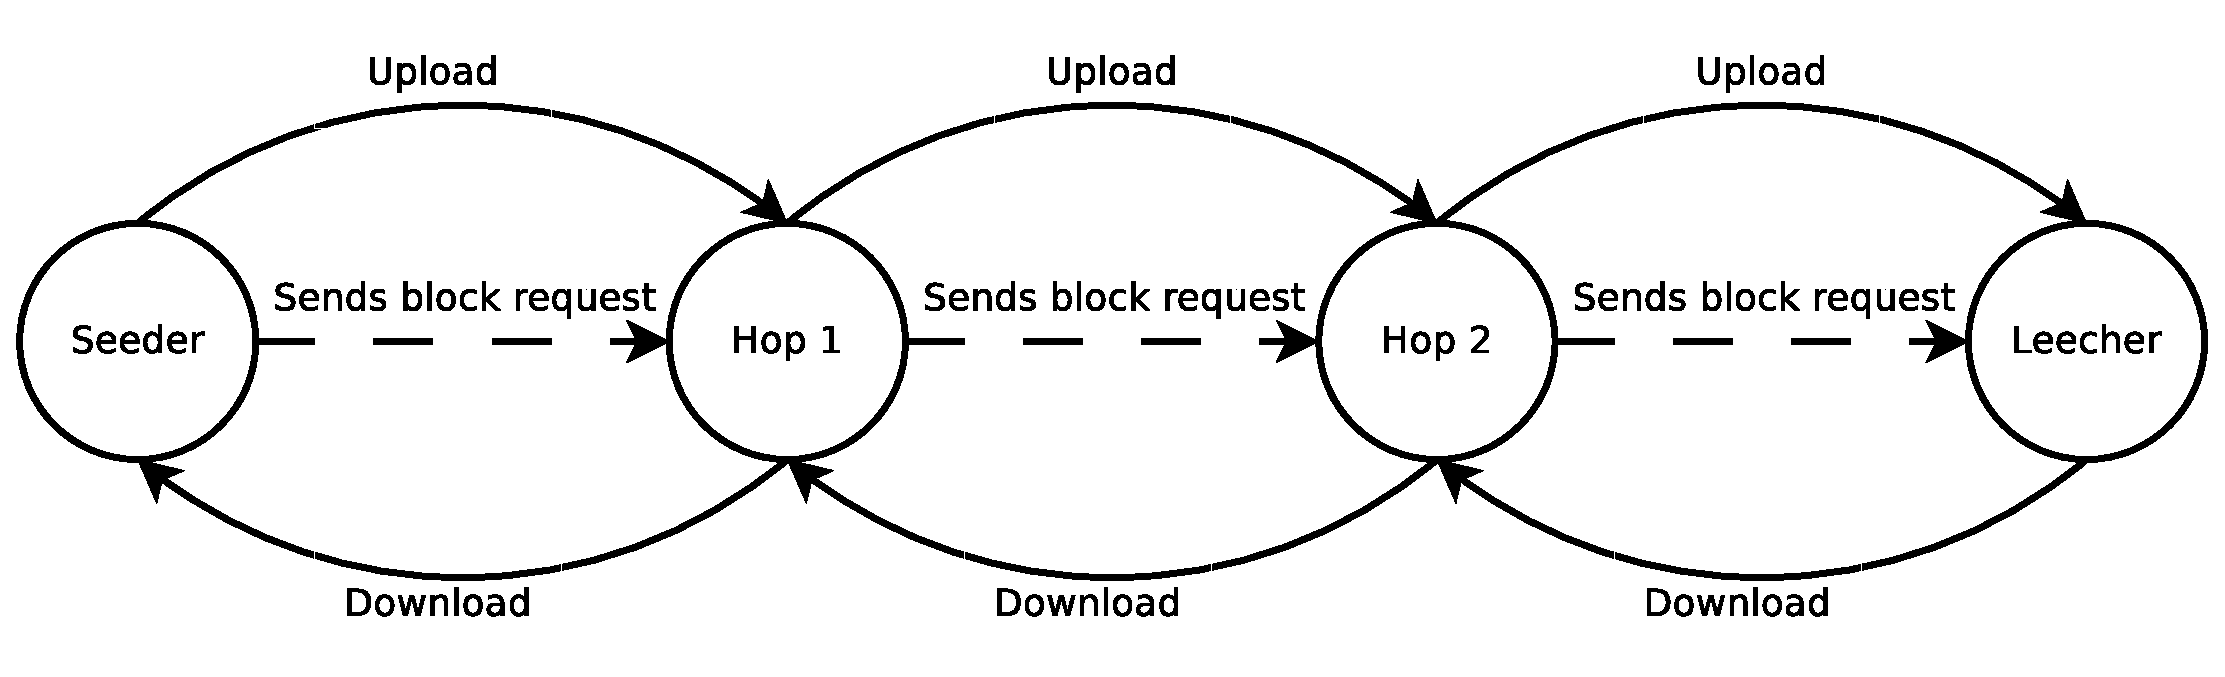
\includegraphics[scale=0.3]{experimentation/anonymous/seeder-hops-leecher.eps}}
	\caption{Block creation in an anonymous download.}
	\label{fig:seeder-hops-leecher}
\end{figure}

The total download and upload amount is plotted, in the same way as the previous experiment,
in Figure \ref{fig:synthetic-anonymous-amounts}.
The slopes of the figures are not representative for the upload and download speeds of the peers.
This is because the x-axis represents the sequence-number of the block and not time.
The hops create blocks that can be categorized in two types:
a download validating block and an upload validating block.
The download validating block only contains information about how much the hop has downloaded
and is initiated by the peer in front of the peer in the sequence.
An upload validating block is initiated by the peer itself with the peer next in the sequence.
The seeder only has upload validating blocks and as such has half the amount of blocks.
The downloader has viceversa only download validating blocks.
The slope of his figure is much steeper as a result.

In the plot a discontinuity can be found at 92\% of the download in the figures of the seeder and the first hop.
This is the result of the first hop sending a signature request to the second hop.
The second hop was not able to process this request,
because it was already working on creating another block.
The second hop drop this request.
The first hop will still wait on the second hop to process its request until it will timeout.
In turn, the seeder sent a request to the first hop that will timeout,
because the first hop is not able to process this request aswell.
During the timeouts of the seeder and the first hop,
the second hop continues to validates its own upload amounts.
No blocks are created that validate his download amount,
so the slope becomes steeper during that time and the download amount remains level.
The timeouted peers create no blocks.
When the timeouts expires, the system returns to function as normal.
In section \ref{sect:deadlock-exp} we further experiment with the timeouts in the system.

\begin{figure}
\centering
\subfigure[Total download amount.]{
\centerline{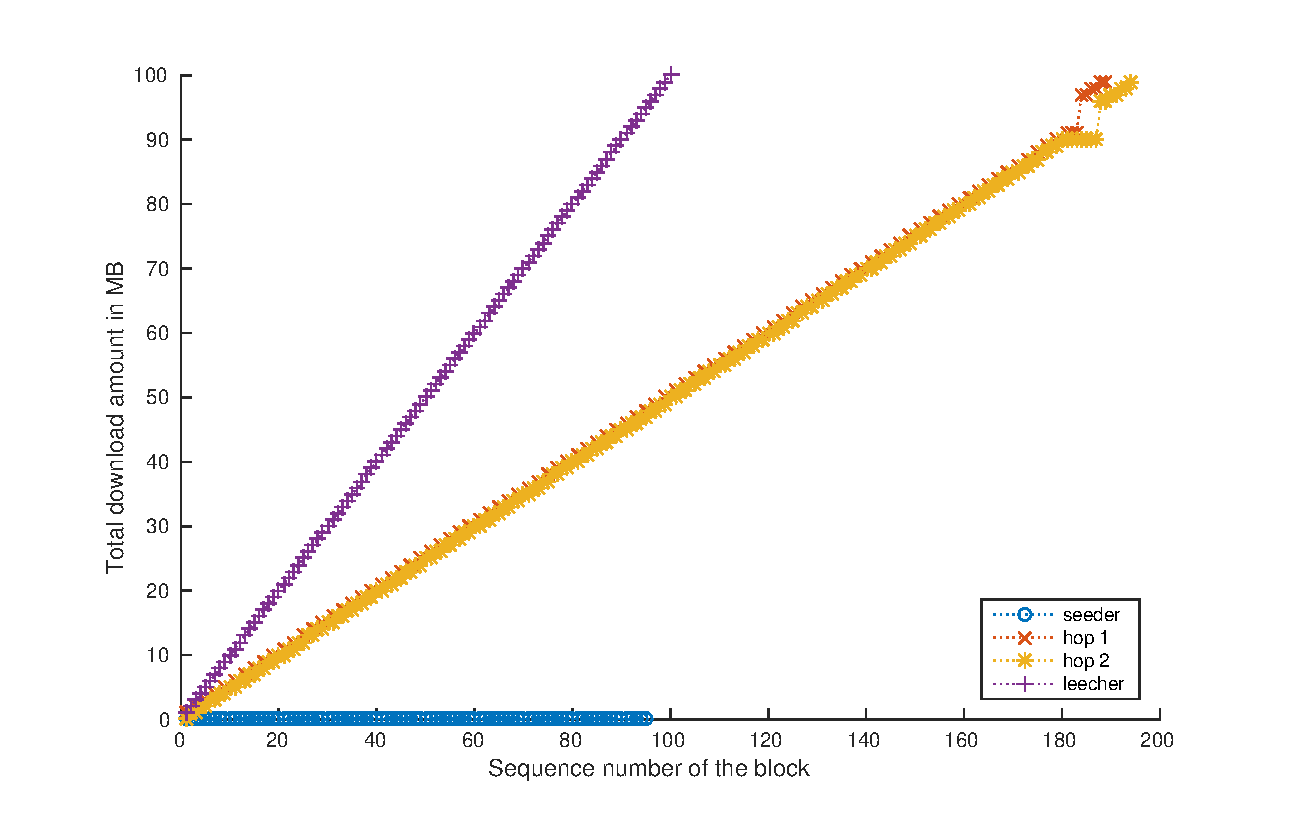
\includegraphics[scale=0.5]{experimentation/anonymous/synthetic-anonymous-down.eps}}
\label{fig:synthetic-anonymous-down}
}
\subfigure[Total upload amount.]{
\centerline{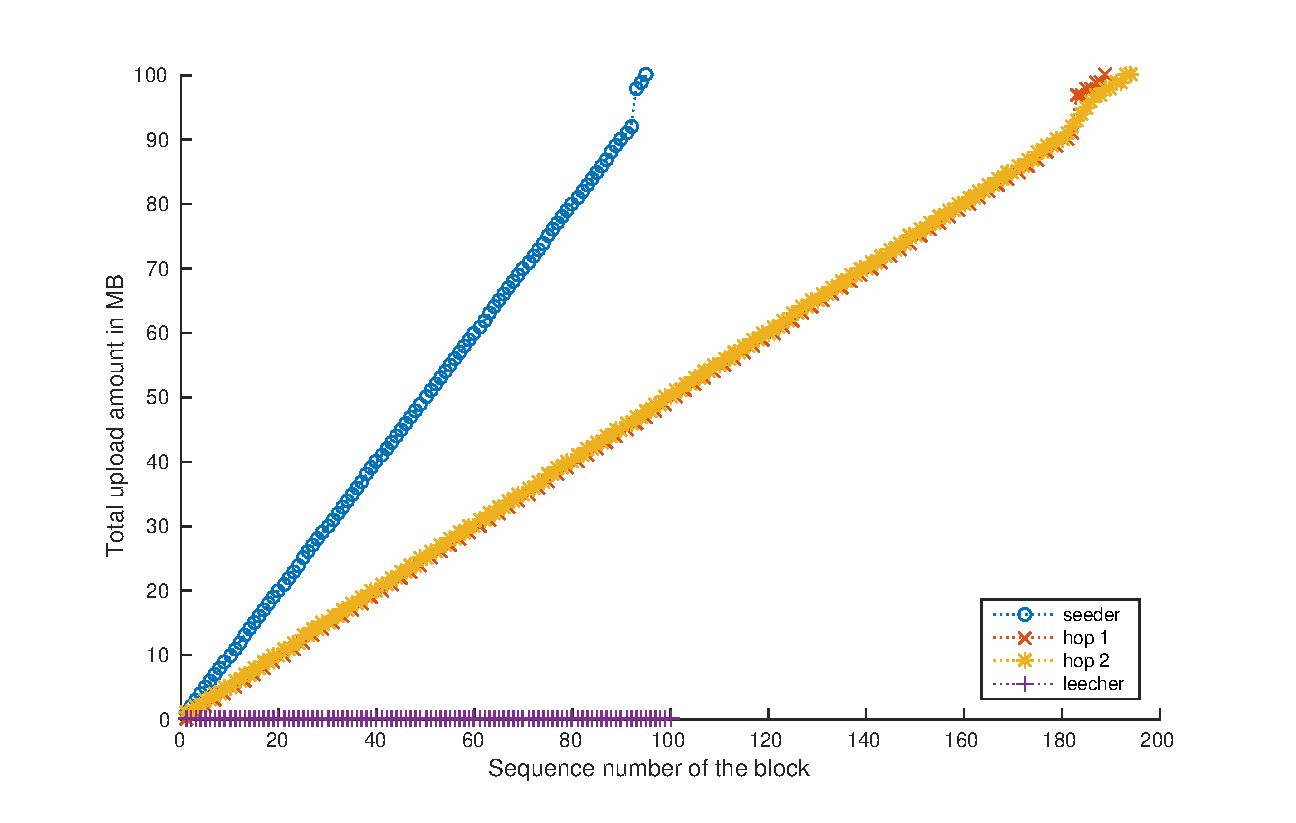
\includegraphics[scale=0.5]{experimentation/anonymous/synthetic-anonymous-up.eps}}
\label{fig:synthetic-anonymous-up}
}
\caption{Download and upload amounts during the anonymous download experiment.}
\label{fig:synthetic-anonymous-amounts}
\end{figure}

The seeder and leecher both only interact with one hop.
These hops furthermore only interact with each other.
This can be clearly seen in a part of the graph magnified in Figure \ref{fig:synthetic-anonymous-graph-magnified}.
The middle nodes represent the interaction between the hops.
The outer nodes are interactions between the seeder and the first hop and between the second hop and leecher.
The blocks are created alternating resulting in the graph pictured.

\begin{figure}
\centering
\subfigure[Partial example of expected MultiChain graph.]{
\centerline{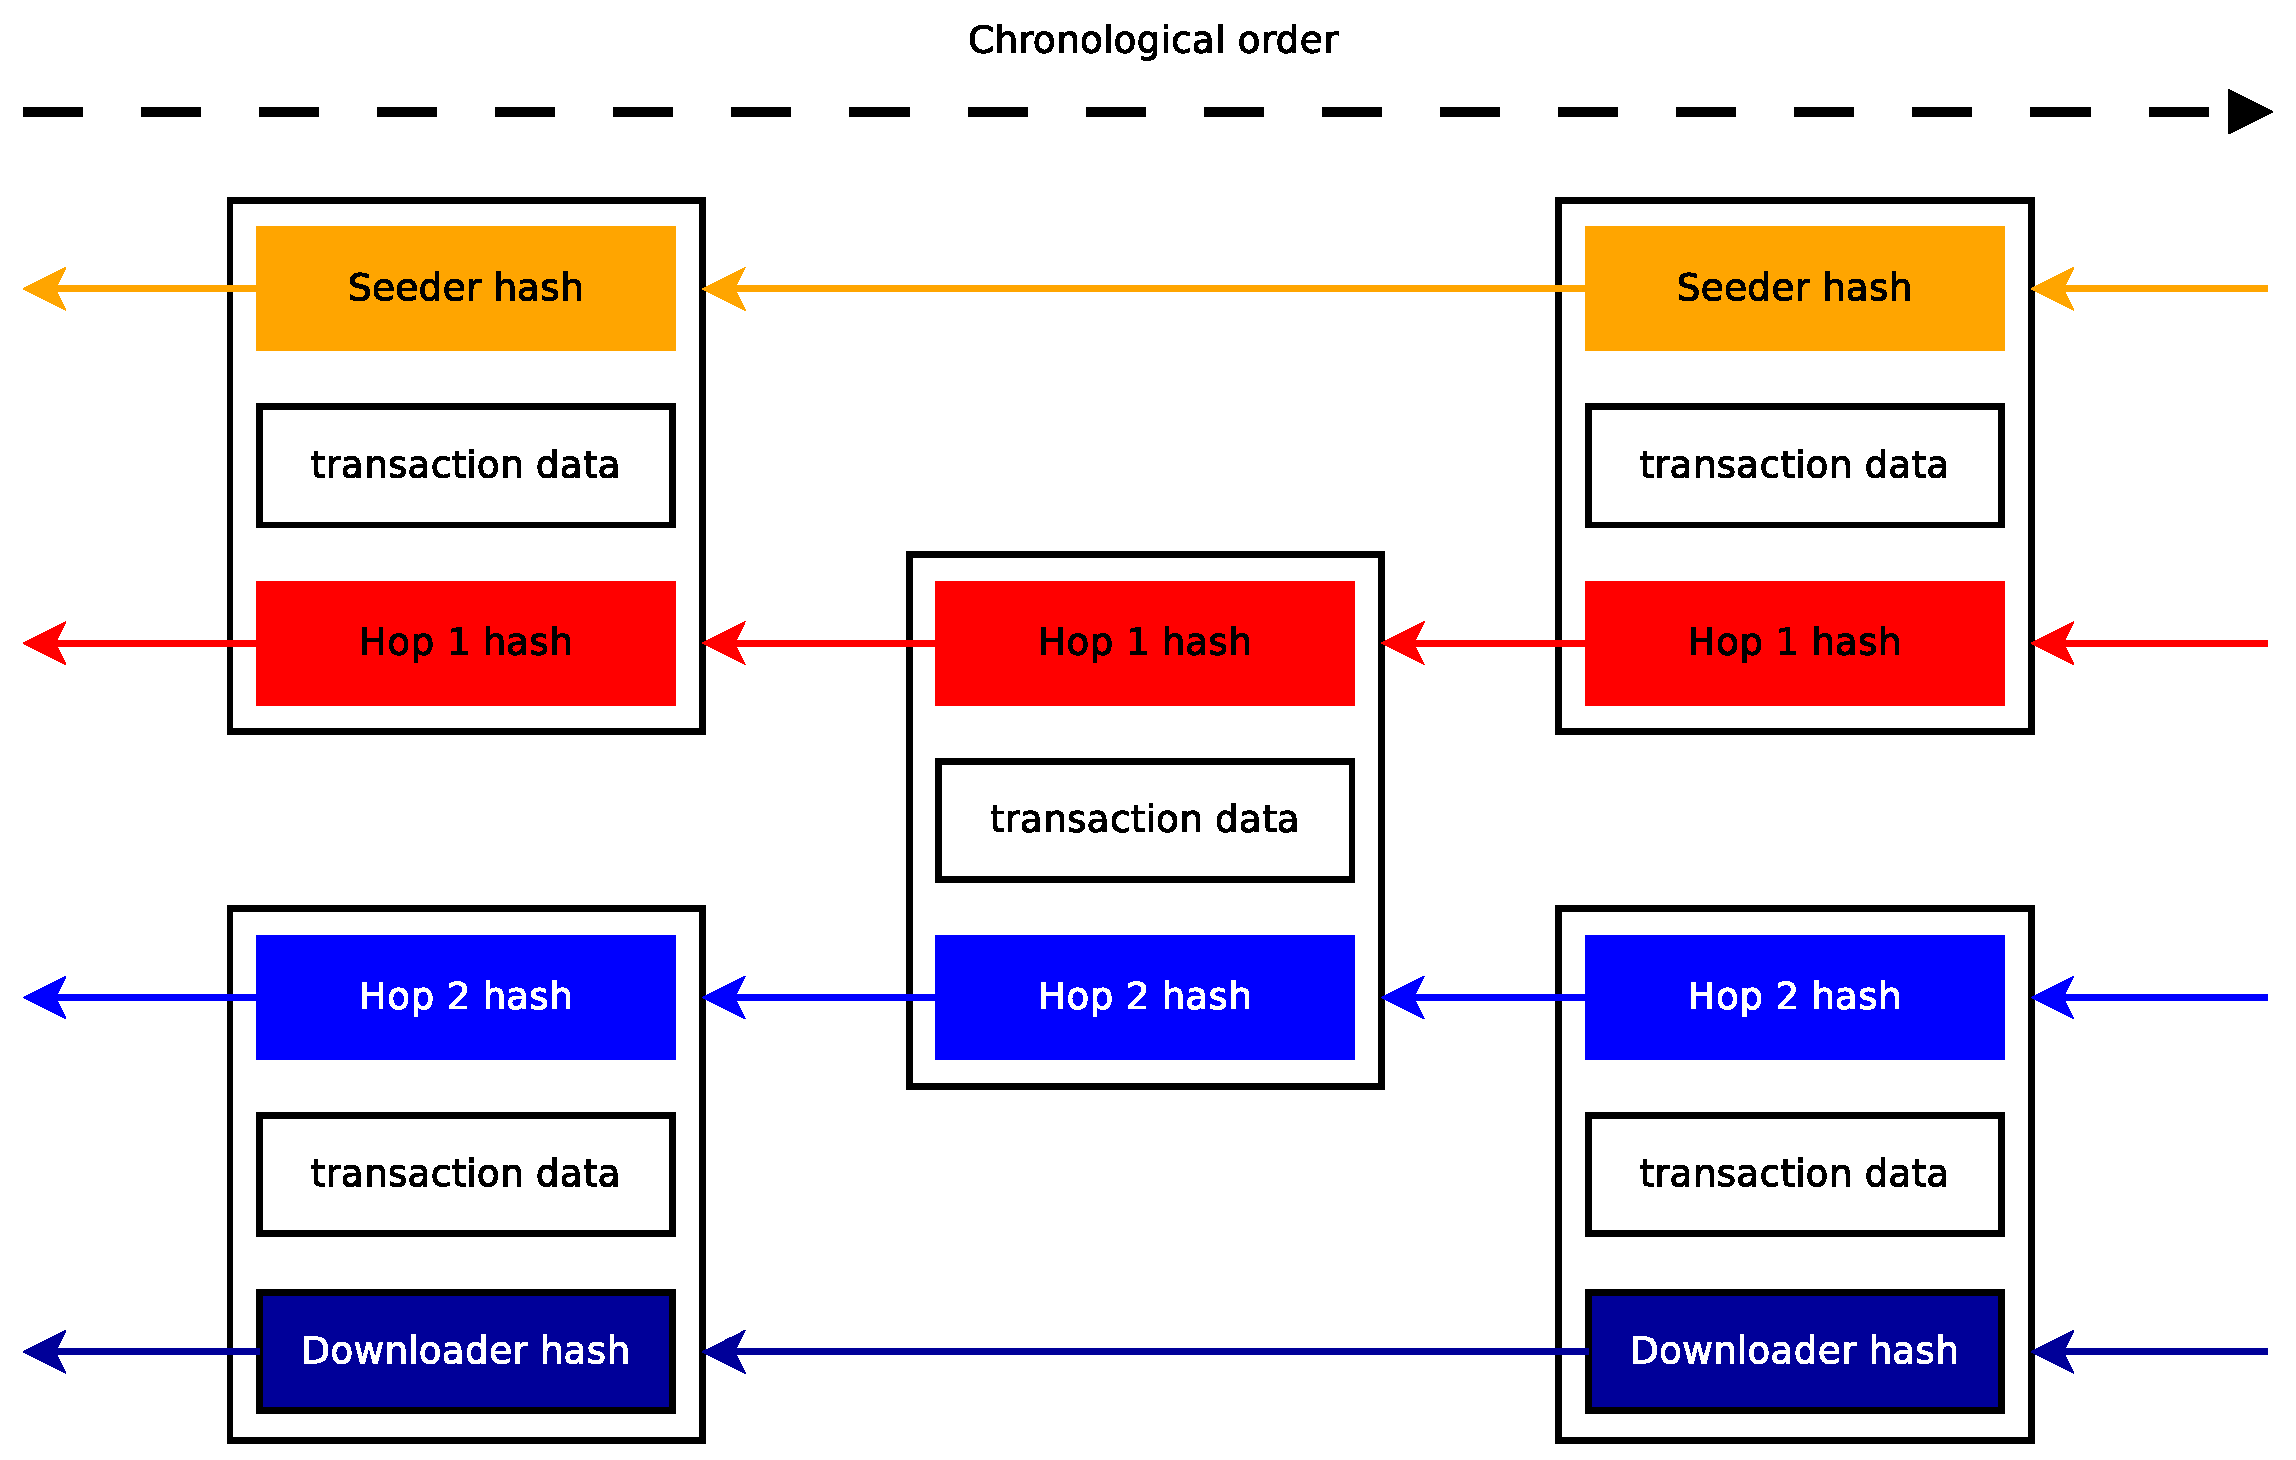
\includegraphics[scale=0.35]{experimentation/anonymous/graph-example.eps}}
\label{fig:synthetic-anonymous-graph-example}
}
\subfigure[Zoom of the actual intertwining in the MultiChain graph made with Gephi.]{
\centerline{\includegraphics[scale=0.2]{experimentation/anonymous/anonymous-magnified.png}}
\label{fig:synthetic-anonymous-graph-magnified}
}
\caption{Intertwining of the seeder and hop 1, hop1 and hop 2, and hop 2 and the downloader.}
\label{fig:synthetic-anonymous-intertwining}
\end{figure}

In the graph the timeout period can be seen clearly in Figure \ref{fig:synthetic-anonymous-timeout}.
The two half-signed block can be seen in red.
The block with a reference coming from the outer block is the half-signed block belonging to the seeder.
The strain of blue nodes are the blocks created between the second hop and the leecher.
The red inner block is referenced by the first block created between the first hop and second hop after the timeout.

\begin{figure}
	\centerline{\includegraphics[scale=0.1]{experimentation/anonymous/anonymous-timeout.png}}
	\caption{Zoom of the timeout of the seeder and hop 1, while hop 2 and the leecher continues.}
	\label{fig:synthetic-anonymous-timeout}
\end{figure}





\section{Deadlock recovery}
\label{exp:deadlock}
MultiChain can run during normal operation into a situation
where two peers are both waiting on each other.
This could resulting in a deadlock.
This situation was encountered during experimentation
and the experiment shows MultiChain correctly recovering from this situation.

In the experiment a 100 megabyte file was downloaded anonymously with 2 hops.
Anonymously downloading is decribed more in the thesis report of R. Ruigrok\cite{ruigrok-anonymous}.
There are 2 Triblers instances with exit functionality and 18 instances without exit functionality.
All instances are run locally on one machine.
The instances are run in parallel,
so the fact that all instances are run on a single machine does not cause the deadlock to occur.
There is no packetloss in this experiment.

The corresponding graph of all the MultiChains of the experiment can be seen in Figure \ref{fig:deadlock-double}.
In this graph the blocks are depicted as nodes and the previous hash pointers are edges in the graph.
The nodes have added colouring to indicate extra meaning.
Green nodes are a first block in a MultiChain of a peer.
Blue nodes are a sequential block between the same previous peers.
Red nodes are half-signed blocks.

The potential scenario of two peers both waiting can be seen multiple times in the graph and are encircled.
The scenario generates a half-signed block at both peers.
Usually the peers continue collaboration and this continuation of a sequence can be seen in subsequent blocks.
In the graph a more complicated scenario can also be seen where multiple peers timeout between each other.

\begin{figure}
	\centerline{\includegraphics[scale=0.0375]{experimentation/deadlock/deadlock.png}}
	\caption{Potential deadlocks in MultiChain.}
	\label{fig:deadlock-double}
\end{figure}


\todo{Move to design}
When MultiChain has a pending signature request,
then it itself will not respond to incoming signature requests from other peers.
These peers themselves will also not respond, because they are not responding to requests for the same reason.
During seeding the seeder will mostly initiate signature requests to the downloader,
but the downloader will have some signature requests for metadata that he sents to the seeder.
These signature requests can be sent in such away that both sent the request before the other receives it.
Both peers are now waiting for the other to respond to the signature request and
will not answer the other resulting in a potential deadlock.
This deadlock can occur between two peers,
but can be expanded into a multiple of peers where each peer waits for another peer in a cycle.

MultiChain prevents this deadlock to occur
by allowing a transaction to fail as explained in section \ref{des:halfsigned}.
If MultiChain gets into this potential deadlock one of the peers will eventually time out of their own signature request
and process the incoming request.
The deadlock is recovered and both peers can continue operation.



%Problems
\chapter{Known vulnerabilities}
\label{problems}
There are several known security vulnerabilities with the current design.
As said in section \ref{pb-aim}, an incremental approach was taken.
As such, the design is part of a bigger system that as a whole is to be developed,
before it can be deployed in the real world.
The current implementation is not yet ready to fully replace BarterCast as a reputation system.
It is too vulnerable for malicious nodes to attack the system.
In this section we will describe the known vulnerabilities
and explain the future work that is needed to limit these vulnerabilities.

\section{Branch attack}
\label{sect:branch}
In this section we will explain an attack that can be done by a malicious node M.
The attack consists of obscuring a part of his transaction history.
M creates a new branch of his transaction history that is more favourable to him.

\subsection{Alternating partial transaction history}
A malicious node M has his own chain of transactions
and he wants to falsify his transactions after a certain point.
He wants to rewrite his transaction history from that point and create an alternate transaction history.
M wants to do this to whitewash his reputation.
The node can simply choose to forget and obscure blocks after that point.
A new branch will be created by chaining new blocks to the desired point in history.

\begin{figure}
	\centerline{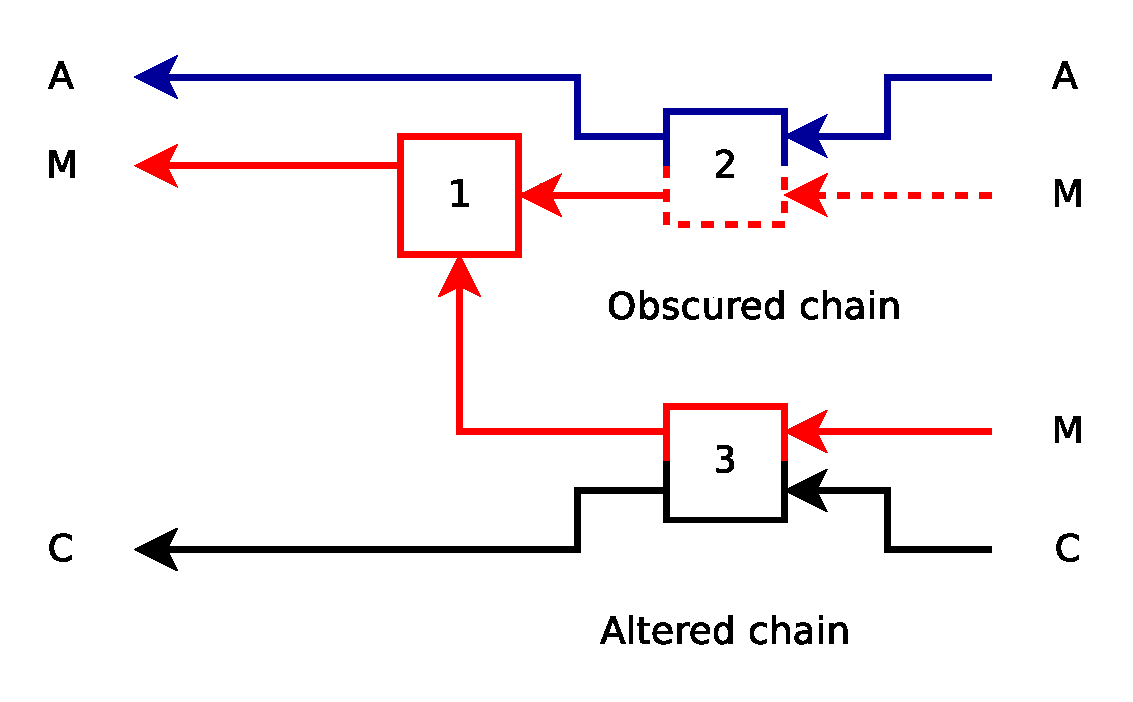
\includegraphics[scale=0.3]{problems/figs/branch.eps}}
	\caption{Example of a branch created by M.}
	\label{fig:problem-branch-obscure}
\end{figure}

In Figure \ref{fig:problem-branch-obscure} an example can be seen of a branch created by M.
In this example M tries to obscure block 2 and any subsequent blocks from C.
When C requests the transaction history of M, M will only send the transaction history up to block 1.
When M and C create a block together,
M will reuse the hash of block 1 in the new block.
For clarity of the diagram, the node interacting with M in block 1 is not displayed.

Now malicious node M does have the problem that not only he knows his transaction history.
When M interacted with node A a block was created that M tries to obscure.
A has this block in his own chain
and therefore knows about it being part of the transaction history of M.
This can be seen in the example in Figure \ref{fig:problem-branch-obscure}.

M will want to reduce the likelyhood of the detection of his fraud.
If his fraud is detected, he might be punished and no longer to continue his abuse.
The first way to minimize detection is to choose
to only interact with new nodes that do not know about the alternate part of the transaction history.
Nodes that have requested an alternate part of the transaction history
or that have been interacted directly with are no longer interacted with.
In a sufficiently healthy network this will result in node M being able to find new nodes to help him.

\begin{figure}
	\centerline{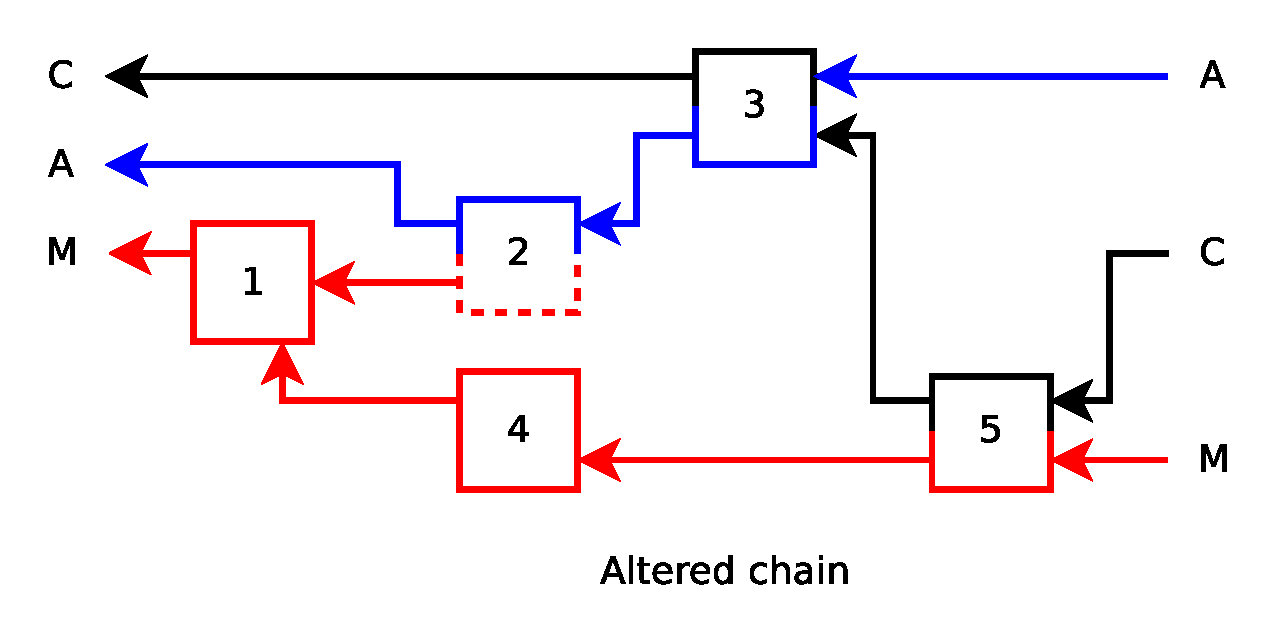
\includegraphics[scale=0.3]{problems/figs/branch-fraud-detected.eps}}
	\caption{Detectable fraud by C.}
	\label{fig:problem-branch-preknowledge}
\end{figure}

There is another example that will expose the fraud of M.
This example can be seen in Figure \ref{fig:problem-branch-preknowledge}.
A node C might still exposes the cheating of M by chance.
C can have an interaction with node A by coincidence.
Before creating block 3 C will request the transaction history of node A containing an obscured block of M.
Now when M wants to interact with C, M will want to create block 5.
When C requests the full transaction history of M, it will detect that the transaction history of M no longer contains block 2.
This exposes the fraud of M.

But C will have no sure way of exposing this type of fraud by his own doing,
except for requesting every transaction history of every node in the system.
This is in a way a common, full transaction history and was chosen to be avoided by the design to become more scalable.
C can limited the possibility of the attack by increasing his knowledge by collecting more transaction history of other nodes.
If node A or B stop participating and exit the network,
then C will have no way of detecting the fraud by M.

The second way M can limit the exposure of his cheating is in a more sophisticated way.
He can present several, different transaction history to different nodes.
M will continue keeping track of the unmodified transaction history.
When M wants to interact with A or B, both knowing this transaction history, he will present this transaction history.
So M can still interact with A and B.
But when interacting with C he will present his alternate transaction history.
C will only expose the fraud in the same way as previously.

This attack can always be done M and is not limited to circumstances.
Also the attack is not limited and M can try to fool any number of other nodes C.
As shown in Figure \ref{fig:branch-multiple}.

\begin{figure}
	\centerline{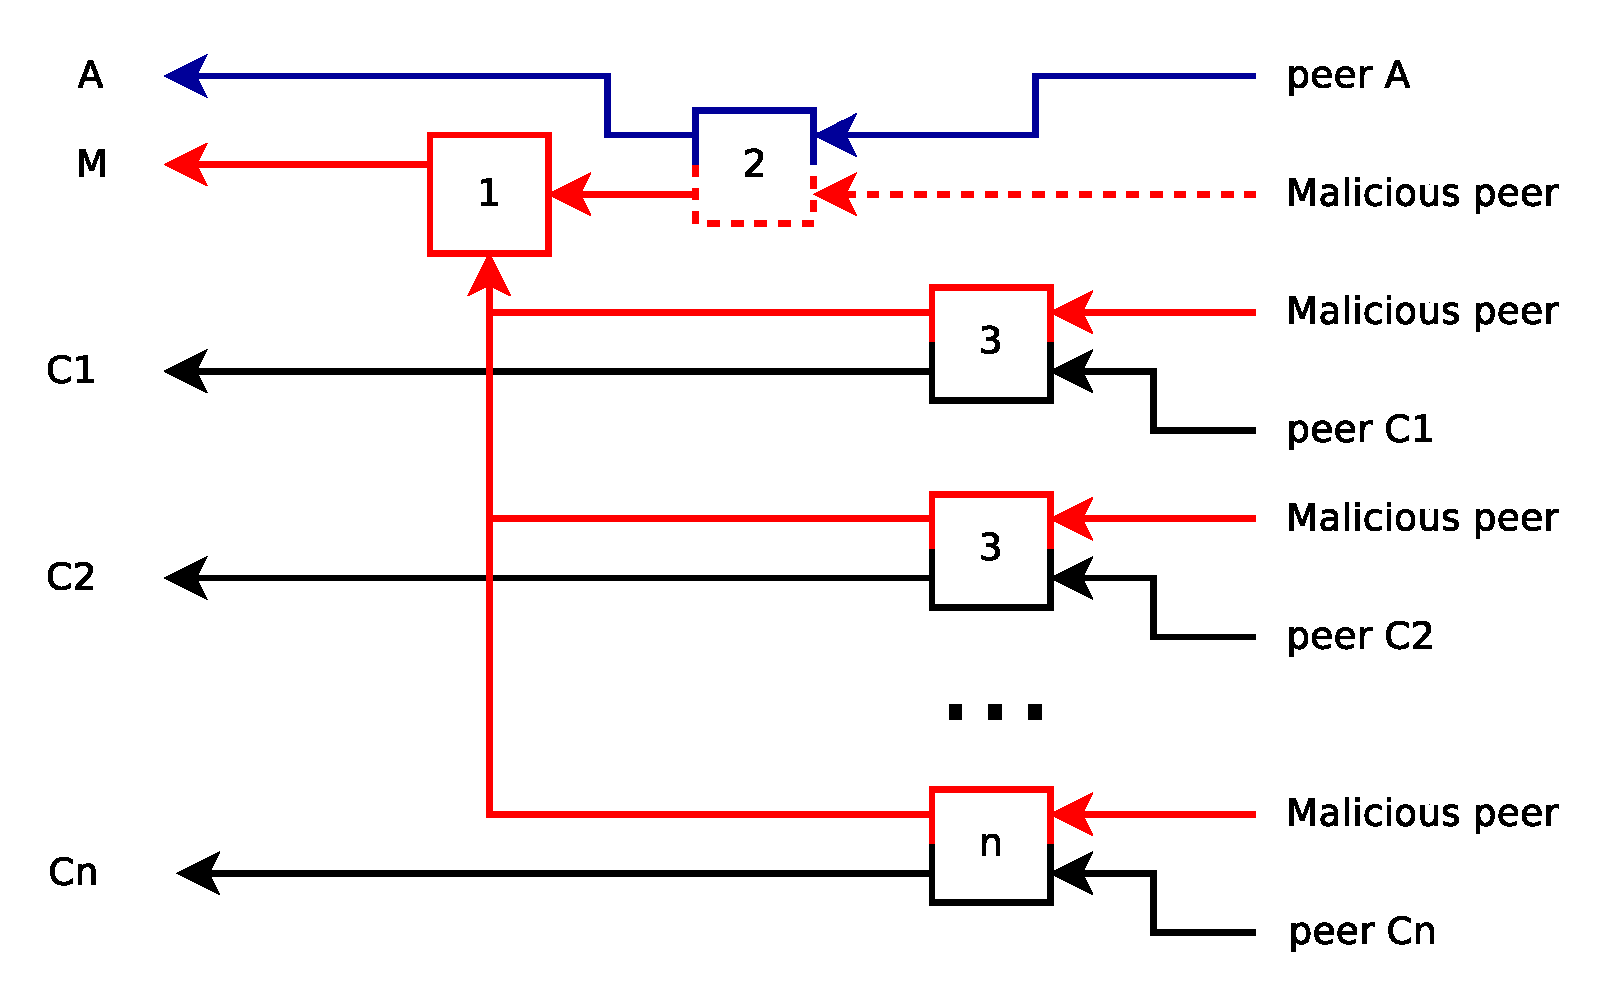
\includegraphics[scale=0.3]{problems/figs/branch-multiple.eps}}
	\caption{Example of multiple branches created by M.}
	\label{fig:branch-multiple}
\end{figure}

The likelyhood of exposing this attack depends on several factors
and will be the only factor to limit M in performing this fraud.
The likelihood depends on:
\begin{itemize}
\item Size of the network
\item Likelihood of interactions between A or B and C
\end{itemize}

These properties will influence the chance of C coming across an obscured block.

\subsection{Punishment of this attack}
When the fraud is detected by C, then currently only C can punish M by no longer interacting with him.
There is currently no way of making it globally known to every node in the network that fraud was committed.
So only M is punished by C and can continue his abuse of other nodes in the network.

A proposal for the future, that is already currently worked on, is to construct an additional network
where the discovery of the fraud can be announced.
Proof of the fraud is easily to distribute and cannot be repudiated by the malicious node.
The proof of the fraud is two blocks containing the same previous hash.
The proof cannot be repudiated, because it contains two signatures by the malicious node.
See section \ref{sect:repudiation} for more explanation.
To increase the likelyhood of detection every node will walk the network to look for fraud.
\section{The Sybil attack}

In this section we will explain the Sybil attack\cite{douceur-sybil}
and how it can be used in the MultiChain system to create an artificial reputation.
An universallly applicable solution has not yet be found\cite{levine-sybilsurvey}.

\subsection{Using fake indentities}
In large distributed systems convincingly distinct identities can be presented
that are infact all under the control of a single adversary M.
Identities can be public keys like in the Dispersy system
or other abstractions of information without direct physical knowledge.
These identities can participate in the system acting like normal agents,
but they can also help each other malificiently to boost each other towards a common goal.

In the MultiChain system the attack is done in the following way.
M creates several other identities besides his own.
This involves generating several key pairs.
Now M controls several identities that can be presented convincingly.
The key pairs do not have to be linked to a node responding to requests.
Failure of nodes are typical in large distributed systems.

Using these key pairs M can now generate an artificial reputation.
Transactions between M and the fake identities are generated by M.
These are signed using the keys of the fake identities.
Using a single transaction it cannot be determined if it is between two distinct identities or a single distinct identity and a fake identity.

\begin{figure}
	\centerline{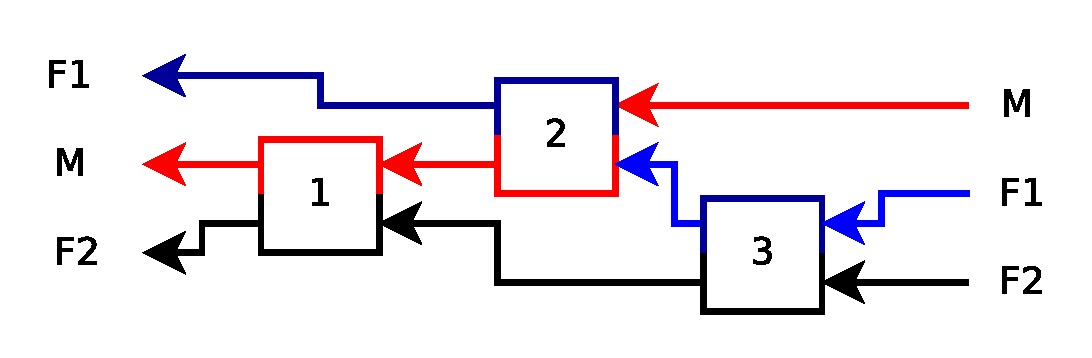
\includegraphics[scale=0.3]{problems/figs/sybil.eps}}
	\caption{The sybil attack by M.}
	\label{fig:sybil-example}
\end{figure}

An example of the Sybil Attack can be seen in \ref{fig:sybil-example}.
In this example M is the malificient node and F1 and F2 his fake identities.
Block 1 and block 2 contain a transaction that is favourable to M,
but M has done nothing to deserve these.
Similair blocks like block 3 can be generated between fake identities in an effort to thwart efforts to analyse the network
and detect fake identities.

In this way M is able to boost his reputation without much work.
The more sophisticated the generation is done by M,
the harder it will be to detect that M boosted his reputation using fake identities.
M can then abuse his fake reputation by solliciting cooperation from other nodes in the network.
They will respond positively on the request by M based upon the false reputation M claims to have.

\subsection{Validating Identities}
A node can have three potential sources of validation of distinct identities:
\begin{itemize}
\item Itself
\item Other entitites
\item A trusted, central authority
\end{itemize}

A node itself could try to directly validate two identities to be distinct.
It would challenge several identities to complete a task that only two entities could complete.
The task would require more resources then a single entity possesses and will be issued simultaneously to all identities.
If the identities complete the task, they have proven to be distinct.
Example of required resources are communication, storage and computation.
These challenges can scale to validate more entities at once.

Indirect validation can be used by a node to by delegating validation to other entities.
A node could accept additional identities to be distinct when an accepted identity vouches for it.
The node has the delegated responsibility to challenge the entity with a challenge.
This would limit the total amount of challenges needed.
But an obvious pitfall of delegating this to other identities is that these can vouch for fraudelent identities.
Next to this, it involves an increase in complexity as the challenges still have to be issued concurrently.

But these challenges are highly indesirable.
These challenges require by definition to occupy between two nodes a limited resource to the maximum capacity of a single node.
While not providing any additional functionality beyond asserting distinct identities.
These challenges also prove inworkable when entities have hugely different amount of resources available.
No challenge can be constructed that can be worked by less powerfull devices,
that could not be worked several times by more powerfull devices.

Next to this, these challenges are only usable with nodes that are active and responding to challenges.
If a node becomes inactive it cannot be ascertained if the node is a fake identity.
But this identity still makes claim about a reputation of another entity.
A choice has to be made between either not counting these claims and allow for a drop in reputation of a node or
allow claims that cannot be validated to be taken into account.
Both options lower the usability of the system.

A trusted, central authority would be able to vouch for distinct indentities
if it has an other way outside the system of asserting that it indeed is a distinct identity.
Approaches exists that implicitly rely on the authority of a trusted agency.
But a central authority goes against the principles of a peer-to-peer network.

Several other defenses against the Sybil Attack have been proposed\cite{newsome-sybil}\cite{dinger-sybil}
or variants on the defenses stated here\cite{levine-sybilsurvey}.
But these either have the same limitation and are minor improvements or are non-applicable for MultiChain.

\subsection{Possibility of attack and likelyhood of detecting fraud}
For M to conduct the Sybil Attack he will need to generate a set of key pairs.
This is trivial to do and Dispersy provides functionality to do this very easily.

\todo{Timing of generating several keys}

With these keys M has to generate blocks.

\todo{timing of generating blocks}

Sybil Attack can have a wide range of sophistication.
Ranging from a large amount of fake identities with a large amount of transaction between them
to a single, fake identity boosting the reputation of M in a couple of transaction.
Even these simple Sybil Attack are hard to defend against if these are not done to obviously.
\section{Denial of service attack}
The denial of service attack is a common attack seen on the internet
that disables a service by flooding it with requests of service.
This is also a potential attack on MultiChain particulairly because of a potential bottleneck.

\subsection{Mutual exclusive code}
A node can only perform a single operation at a time on its chain.
Multiple blocks cannot be created because they will both point to the same block and create a block.
This can be seen as an attack and should be punished as described in section \ref{sect:branch}.
So safeguards have been implemented to ensure that this does not occur.

This was done by implementing mutual exclusion for code that creates a block.
Only one block creation operation can be pending at any time.
This can be either requesting to create a new block with another peer and wait on response or
processing a request itself.
Because only a single operation can be handled at one time
this makes a node very vulnerable to a denial of service attack.
A bottleneck is introduced by design that cannot be scaled.

If a node is flooded by sufficient bogus requests to create a new block,
then it will become over burdend with these requests to service real requests or to send send out its own requests.
The node is denied service and cannot create meaningfull blocks.
Because the node becomes unresponsive to block creation requests other nodes will not trust him to sign future blocks
and will not be granted upload bandwidth.
The other node does not trust that in return he will receive a boost in his reputation and will stop collaboration.
The node under attack will also be unable to transform his own collaboration into a boost in reputation
by sending his own block creation requests.

The proposed denial of service attack is more sophisticated than typical denial of service attacks.
These typicaly involve simply flooding a server with requests,
but for the proposed attack the requests have to be crafted with care.
They need to valid to be serviced by the attacked node and reach the mutual exclusive part
that is the vulnerable bottleneck.
A request has to be a counterpart of a real interaction or the request can be easily filtered.
The filtered request will still impose a computational and network burden on the node,
but this is always a vulnerability and not a specific vulnerability of MultiChain.

\subsection{Filtering requests}

Detection can be implemented that will help in detecting fake requests.
The detection can be run in parallel and does not have to enter the mutual exclusive part.
Any request that is fake will not reach the mutual exclusive part
and will not drown out the service of valid block creation.
Effective analyses have to be researched and implemented in future work to harden the system to this attack.








%Conclusion
\chapter{Conclusion}
A reputation system is a necessity in a collaborative network like peer-to-peer filesharing.
But the creation of a tamper-proof interaction history is a difficult undertaking.
As seen as by several attempts in related work with varying success.
This first step, in an incremental approach to creating a new data structure
that can be used as a tamper-proof interaction history, is further testimony to that statement.
But MultiChain is a proof-of-concept that an different approach with multiple chains
instead of a single chain can be succesfull in creating a reputation system

A scalable system has been introduced that can track interactions.
The system does not rely on any central component or a central data structure.
This system has been succesfully integrated with Tribler.
MultiChain can be released as a first version to start measuring the system in the real world.
Improvements can be implemented using these measurements.

MultiChain has been tested in software engineering tests and experiments.
These tests prove the system to be correctly working as designed.
The experiments show that MultiChain to behave as expected in a real world scenario.
MultiChain tracks the interactions between multiple nodes correctly in these scenario's.

The current implementation is not yet ready to fully replace BarterCast as a reputation system.
It is too vulnerable for malicious nodes to attack the system.
The possibility and impact of these attacks have to be reduced
before MultiChain can be fully used as a reputation system with a reasonable amount of trust.
Proposals are already made and worked on to harden the system in the future.




% BIBLIOGRAPHY
\bibliographystyle{bib/latex8}
\bibliography{bib/bibliography}

%\appendix

%\include{appendix_a}

\end{document}

